%!TEX root = ../../thesis.tex
As mentioned previously, soft robots are composed of soft bodies that may be regarded as a continuum body with (theoretically) infinitely many degrees of freedom (DOF). In this section, we aim to derive a compact and computationally efficient model that envelops the continuous dynamics of a soft robot through a small set of generalized coordinates $\q\in\Q$ and their respective generalized velocities $\dq\in T_{\q}\Q$ with $n$ the number of active joint variables. We base the modeling framework on the work of Mochiyama et al. (2003, \cite{Mochiyama2003}), who outlined a theoretical foundation for continuum manipulators. Their work is extended upon by including extensibility, serial-chaining of multiple soft links, pneumatic actuation, and the introduction of nonlinear and time-dependent material behavior. Earlier modeling strategies addressing similar issues can be found in from Godage et al. (2016, \cite{Godage2015,Godage2016}), Della Santina et al. (2020, \cite{DellaSantina2020,DellaSantina2020a,DellaSantina2021}), Renda et al.
(2018, \cite{Renda2018}), and Boyer et al. (2021, \cite{Boyer2021}). Leveraging from the aforementioned works, the continuous dynamics of a soft robot manipulator can be written in the familiar Lagrangian form:
%
\begin{align}
\MB(\q) \ddq + \vec{h}(\q,\dq) & = \vec{J}^\top\!(\q) \vec{\lambda} + \vec{\tau}(\q,\vec{u}), \label{eq:C2:model0}\\
\vec{\tau} & = \vec{G}^\top\!(\q) \vec{u}.
\label{eq:C2:input_model0}
\end{align}
%
where $\MB(\q) \in \R^\nn$ denotes the generalized inertia matrix, $\vec{h}(\q,\dq) \in \R^n$ a vector of nonlinear state-dependent force contributions. The nonlinear state-dependent contributions possess a structures as follows: $\vec{h}(\q,\dq) = \vec{C}(\q,\dq)\dq + \vec{f}(\q,\dq)$ of Coriolis forces and visco-elastic terms, respectively.

\begin{asm}[Finiteness generalized inertia]
The inertia matrix is a positive definite symmetric matrix that is bounded from both sides $\lambda^{-} \preceq \mat{M}(\q) \preceq \lambda^{+}$ for all configurations $\q$.
\end{asm}

\begin{asm}[Passivity]
For any velocity $\dot{\q}$, it holds that $\dot{\q}^\top\left(\dot{\mat{M}} - 2\mat{C}  \right)\dot{\q} = 0$ -- the so-called passivity condition for Lagrangian systems. If the condition holds, it can easily be shown that map $\uB \mapsto \dot{\q}$ is passive, which implies that there exist a constant $\beta \ge 0$, such that the energy produced by the system $E^{\textrm{u}}$ bounded from below \cite{Ortega1998}:
%
\begin{equation}
E^{\textrm{u}} := \int_0^T \dq^\top(\tau) \uB(\tau) \;d\tau > -\beta \quad \forall\,T > 0.
\label{as:C2:passivity}
\end{equation}
%
\end{asm}

\begin{asm}[Under-actuation]
In many cases, a soft robot that falls under the category hyper-redundant is also intrinsically under-actuated. Mathematically, under-actuation is defined as follows \cite{Russ2022}. A second-order system $\ddot{\q} = \fB(\q,\dq,\uB,t)$ is fully-actuated if, for any time $t$ and state $(\q,\dq)$, the flow map $\fB$ is surjective. In laymen's terms, for any acceleration $\ddot{\q}$ there is exists a unique input $\vec{u}$ that produces such response. Otherwise, the system is under-actuated. Given the control affine structure in \eqref{eq:C2:input_model0}, the system is under-actuated if exist configurations $\q \in \Q$
such that $\rank \left( \vec{G}(\q) \right) < \dim(\q)$.
Let it be clear that fully-actuated systems are dramatically easier to control than underactuated systems. However, for the sake of simplicity at this stage, we assume the actuation matrix to be full rank and time-invariant, \ie, $\vec{G}(\q) \equiv \vec{G}$. Under-actuation will be treated further in Chapter 4 and will not be considered in Chapter 3.
\end{asm}

In this chapter, a similar modeling framework is adopted to \cite{Mochiyama2003}; however, we propose an extension to incorporate FEM-driven data to more accurately reflect the underlying continuum mechanics -- in particular, hyper-elasticity and visco-elastic creep. We also propose a numerical scheme that significantly accelerates the computation of the continuous dynamics.

\subsection{Piecewise curve kinematics}
\noindent To represent the hyper-flexible configuration of the soft robot, let us consider a smooth spatial curve that passes through the geometric center of the continuously deformable body, as shown in Figure \ref{fig:C2:configuration}. {In literature, this curve is called} the '\textit{backbone curve}' as it simplifies the three-dimensional deformation imposed by distributed forces acting on the elastic body. The arc-length of the backbone corresponds to the extensible length of the soft robot denoted by the variable $l(t)$ which we assume bounded ${l}_{-}\le l \le {l}_{+}$, and let $L$ be a constant denoting the {total unstressed} length of the soft robot. Next, let us introduce a spatial variable $\sigma \in \Xs$ that belongs to the one-dimensional material domain of the backbone curve, i.e., $\Xs = [0,\, L]$. Let it be clear that the spatial variable $\sigma$ represents the arc-length of a material coordinate along with the undeformed material domain of the soft robot manipulator.

Given each material coordinate, we wish to find a suitable low-dimensional joint representation $\q(t)$ such that the position vector $^0\gammaB$ anywhere on the continuous backbone can be written as a mapping from generalized coordinates and space into Euclidean space $\R^3$:
%
\begin{equation}
^0\gammaB: \Xs \times \Q(\Ts) \to \R^3;
\end{equation}
%
and similarly the rotation matrix $^0\mat{\Phi}(\sigma,\vec{q})$ by a mapping from the generalized coordinates and space into $\SO{3}$:
%
\begin{equation}
^0\PhiB: \Xs \times \Q(\Ts) \to \SO{3}, \label{eq:phi_map}
\end{equation}
%
where {$\SO{3}$ denotes the special orthogonal group for rotations about the origin of $\R^3$}, $n = \dim(\vec{q})$ the state dimension, and the manifold $\Q$ is an embedding of temporal coordinates $t \in [0,T]$. We provided a more detail description on the rotation group $\SO{3}$ in Appendix \ref{app:C2:adjoint}. For sake of brevity, we drop the superscript that indicates the frame of reference, \ie, $^0\PhiB = \PhiB$ and $^0\gammaB = \gammaB$. Under this notion, the position vectors $^0\gammaB(0,\q)$ and
$^0\gammaB(L,\q)$ relate to the base and the end-effector of the soft robot, respectively. {Please note that left-sided superscript are used to indicate the frame of reference.} The set of all points on the backbone
$\vec{\mathcal{C}} = \left\{\gammaB \in \R^3\, |\, \sigma \in \Xs \right\}$ draws a possible {spatial} configuration of the soft robot given {a time instance $t \in \mathbb{T}$ on a finite horizon $\mathbb{T} = [0,T]$}.
%
\begin{figure}[!t]
  \vspace{-0.6mm}
  \centering
  \ifx\printFigures\undefined
  \else
  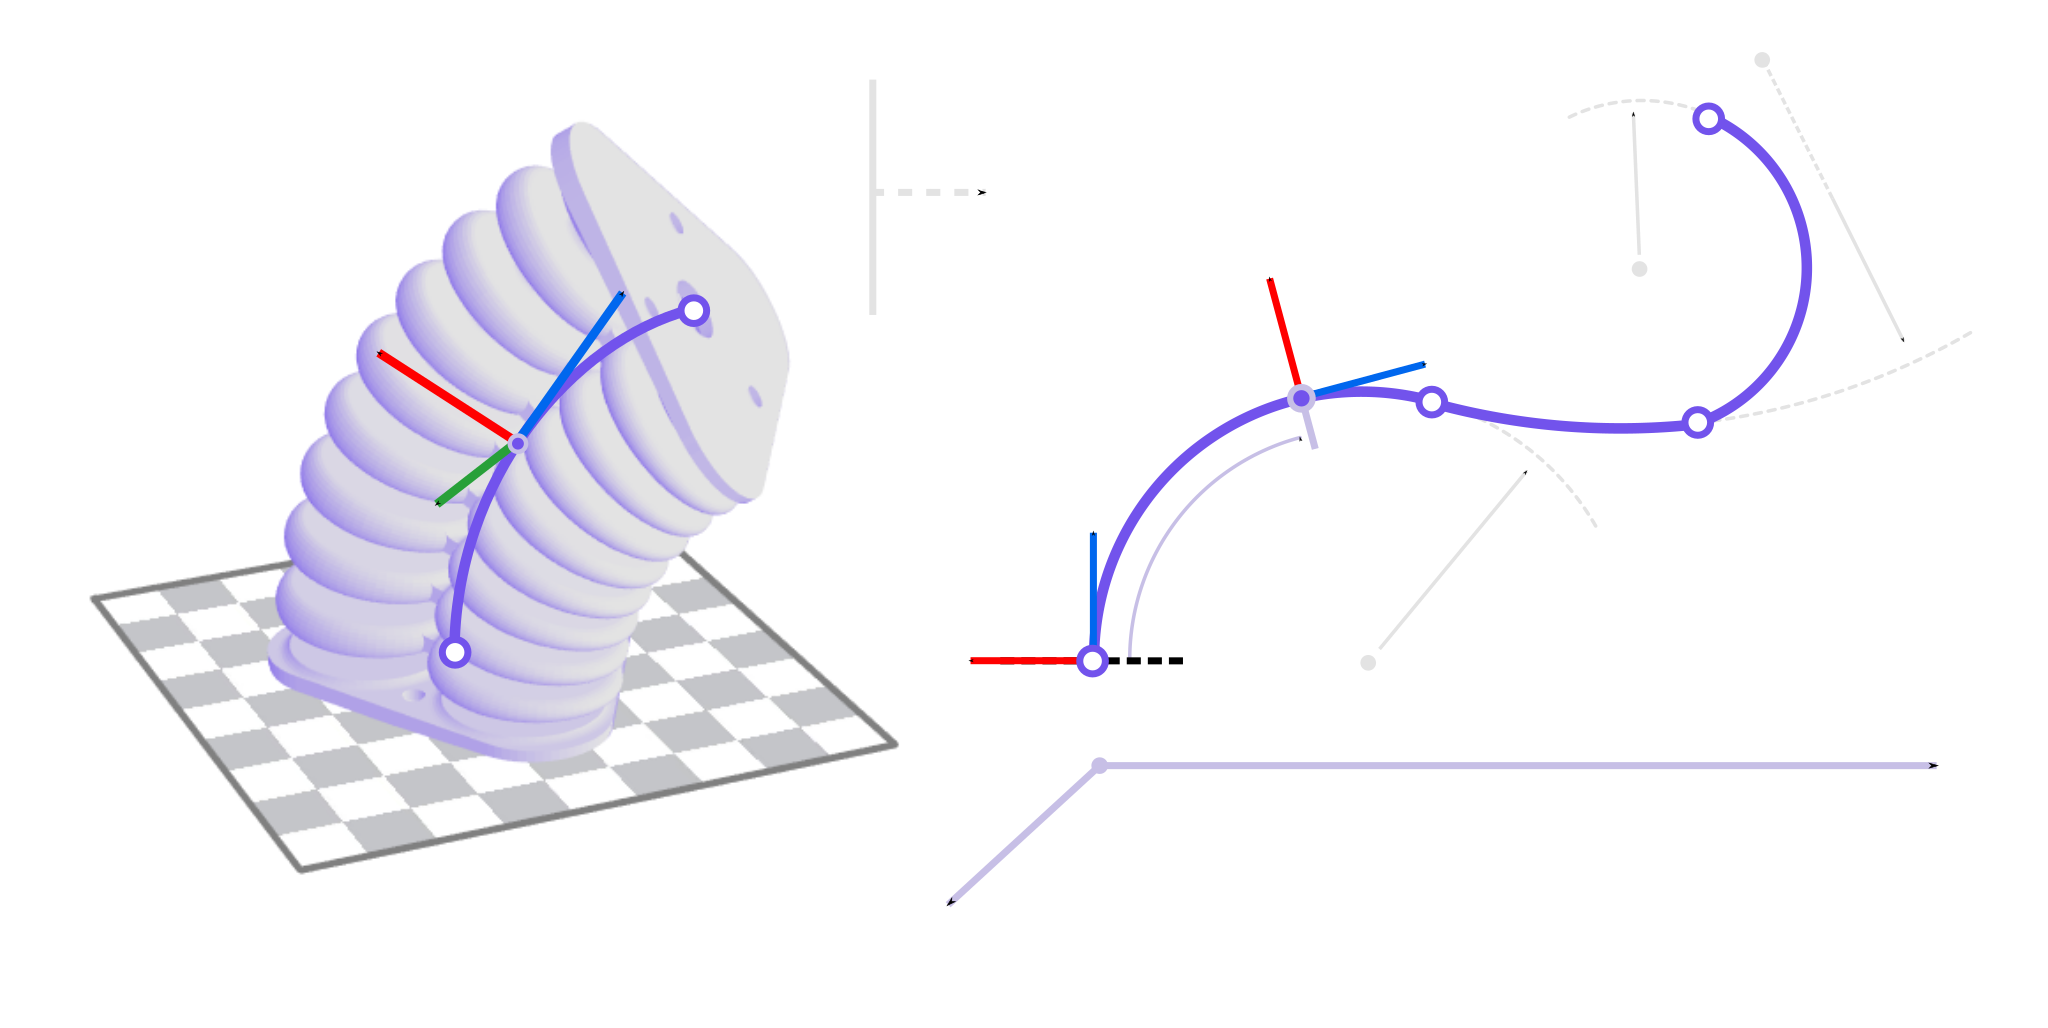
\includegraphics[width = 0.99\textwidth]{fig_C2_schematic.pdf}
  \fi
  \caption{Schematic representation of the Piece-wise Constant Curvature model (PCC) for general soft robotic system, given by a parameterized curve $^0 \gammaB: \Xs \times \Ts \to \R^3$ and orientation matrix $^0 \PhiB: \Xs \times \Ts \to \SO{3}$. The frame $\{\sigma\}$ is rigidly attached to $^0 \gammaB$ such that variation of $\sigma$ give insight into the differential geometry of the curve.}
  \label{fig:C2:configuration}
\end{figure}
%
\begin{dfn}[Piece-wise Constant Curvature]
Despite the inherent flexibility in soft robotics, it is sometimes sufficient to express the kinematics according to the \emph{Piecewise Constant Curvature} (PCC) condition. Mathematically, it implies that the curvature of the continuous body satisfies $\kappa(\sigma_1,\q) = \kappa(\sigma_2,\q)$ for a neighboring region of points $\sigma_1,\sigma_2 \subseteq \Xs$. As a result, this condition allows us to describe the full forward kinematics with a significantly reduced set of generalized coordinates, mitigating kinematic complexity in the model. Numerous works employ PCC models \cite{Falkenhahn2015,Katzschmann2019,Tatlicioglu2007,Marchese2016,Godage2016,DellaSantina2020a}, and depending on the elasticity, the PCC condition has been proven to be consistent for various soft robotic systems.
\end{dfn}
%
{Following this Constant Curvature (CC) description, let us assign a coordinate frame that twists minimally along the backbone -- formally called the \emph{Bishop frame} (see, \cite{Bishop1975}) -- parametrized by the following generalized coordinate vector:}
%
\begin{equation}
\vec{q} := \begin{pmatrix}
\,\varepsilon & \kappa_x & \kappa_y\,
\end{pmatrix}^\top \in \mathcal{Q},
\label{eq:C2:coordinate}
\end{equation}
%
\noindent where $\varepsilon_{-} \le \varepsilon \le \varepsilon_{+}$ is the elongation strain, and $\kappa_x,\,\kappa_y\in\mathbb{R}$ are the curvatures or angular strains in $x$-$z$ and $y$-$z$ plane, respectively; and
$\mathcal{Q} \subset \R^3$ is an admissible space on which $\q$ evolves. Also, we denote the total curvature by $\kappa = \inner{\kappa_x}{\kappa_y}$ together with the curvature angle $\phi = \atantwo(\kappa_y,\kappa_x)$. It is worth mentioning that the joint description above is somewhat related to Renda. et al. (2018, \cite{Renda2018}) who proposed a \emph{Piece-wise Constant Strain} (PCS) parametrization with the exception of including the twist along the tangent.

By exploring the differential geometry of the smooth backbone curve similar to Mochiyama et al. (2003, \cite{Mochiyama2003}), we can write the position vector $\gammaB(\sigma,\q)$ and the orientation matrix $\PhiB(\sigma,\q)$ for each material point $\sigma$ along the smooth backbone as a differential equality of the form:
%
\begin{align}
\renewcommand*{\arraystretch}{2}{}
\frac{\partial \,\!\mat{\Phi}}{\partial \sigma}(\sigma,\q) & = \, \mat{\Phi}(\sigma,\vec{q}) \,\mat{\Gamma}^{\times} (\sigma,\q) \label{eq:C2:change_phi} \\[0.45em]
%
\frac{\partial \, \gammaB}{\partial \sigma}(\sigma,\q) & = \, \mat{\Phi}(\sigma,\vec{q}) \, \vec{U}(\sigma,\q), \label{eq:C2:change_p}
\end{align}
%
where $\vec{\Gamma}^\times \in \SO{3}$ is a skew-symmetric matrix composed of the entries of the vector $\vec{\Gamma} \in \R^3$, and $\vec{U}\in \R^3$ a vector representing the tangent along the extensible backbone. For readers familiar with Lie Groups, the operator $(\,\cdot\,)^\times$ denotes the isomorphism between the Lie algebra $\sog{3}$ and $\R^3$. The vectors $\vec{\Gamma}$ and $\vec{U}$ are vectors that define the differential geometry of the backbone
\cite{Mochiyama2003} which are unique entries that live in the tangent space of the rigid-body transformation group, \ie, $T_{\SE{3}}$. Given the Bishop parametrization as described by \eqref{eq:C2:coordinate} and assuming the Constant-Strain (CC) condition, these geometric entities yield
%
\begin{align}
\vec{\Gamma}(\sigma,t) & \cong \vec{\Gamma}(\sigma,\q(t)) \quad \xRightarrow[]{\textrm{CC condition}}\quad \vec{\Gamma}(\q) = \begin{pmatrix} \;-\kappa_y\;\; \\ \;\kappa_x\;\; \\ \;0\;\;  \end{pmatrix}, \\[0.35em]
%
\vec{U}(\sigma,t) & \cong \vec{U}(\sigma,\q(t)) \!\quad \xRightarrow[]{\textrm{CC condition}} \quad \vec{U}(\q) =  \begin{pmatrix} \;0\;\;  \\  \;0\;\; \\ \varepsilon + 1\ \end{pmatrix},
\end{align}
%
%with $\vec{U}^\circ$ the unit-tangent pointing, and $\vec{\Gamma}^\circ$ the intrinsic curvature/torsion of the curve. For simplicity, lets assume $\vec{U}^\circ = (0,0,1)^\top$ and $\vec{\Gamma}^\circ = \vec{0}_3$.
Now, given an initial configuration of backbone's base, \ie,$\mat{\Phi}(0,\vec{q}) = \vec{\Phi}_0$ and $ \gammaB(0,\q) = \vec{0}_3$, we can now solve for the position and orientation for each material coordinate $\sigma$ along the backbone:
%
\begin{align}
\mat{\Phi}(\sigma,\vec{q}) & = \vec{\Phi}_0\exp_{\SO{3}}(\sigma \vec{\Gamma}^\times(\vec{q})), \label{eq:C2:phi_exact} \\[0.35em]
\gammaB(\sigma,\vec{q}) & = \int_0^\sigma\,^0\mat{\Phi}(\eta,\vec{q})\, \vec{U}(\vec{q}) \; d\eta,
\label{eq:C2:pos_exact}
\end{align}
%
where $\exp_{\SO{3}}: \sog{3} \to \SO{3}$ is the exponential map. Luckily, there exist a compact expression for the exponential mapping related to the orthogonal group of rotation matrices $\SO{3}$ called the \emph{Rodriguez formulas}. Given the rotation angle $\theta(\sigma,\q) := \int_0^\sigma \kappa(s,\q) \; ds = \kappa(\q) \sigma$, we can compactly rewrite the rotation matrix \eqref{eq:C2:phi_exact} in terms of $\cos(\theta)$ and $\sin(\theta)$ using these formulas as follows \cite{Lynch2017}:
%
\begin{equation}
\PhiB(\theta) = \PhiB_0 \left( \mat{I}_3 + \left[ \frac{\sin(\theta)}{\theta} \right]  \GammaB^{\times} + \left[ \frac{1-\cos(\theta)}{\theta^2} \right]  \GammaB^{\times} \GammaB^{\times} \right).
\label{eq:C2:phi_rodr}
\end{equation}
%
We wish to inform the reader that the closed-form solutions \eqref{eq:C2:phi_exact} and \eqref{eq:C2:pos_exact} represent the forward configuration kinematics of the backbone curve. To express the forward velocity kinematic, let
$\etaB(\sigma,\q,\dq) = \left( \vec{\omega}^\top, \vec{v}^\top \right)^\top \in \R^6 \cong \seg{3}$
 be the aggregate of the angular velocity and linear velocity components relative to an inertial frame at $\sigma$, where the space $\seg{3}$ denotes the Lie algebra of $\SE{3}$. The velocity twist is computed by the following integration procedure:
%
\begin{align}
 \etaB(\sigma,\q,\dq) = \Ad_{\mat{g}(\sigma,\cdot)}\inv \int_0^\sigma \Ad_{\mat{g}(s,\cdot)}\, \JB^\star\! \dq\;ds
 \,=:\, \JB(\q,\sigma) \dq, \label{eq:C2:vel_cont}
\end{align}
%
where $\Ad_g: \SE{3} \to \mathbb{R}^{6\times 6}$ denotes the adjoint transformation matrix regarding the rigid body transformation $\gB \in \SE{3}$ that maps local velocities (i.e., twist) to a frame located at $\sigma$, and $\JB^\star:\Q \to T_{\q}\Q$ the joint-axis matrix that relates the DOFs to the geometric deformations. Let it be clear that the joint-axis matrix is naturally constant for a soft segment modeled with the Constant-Strain (CS) assumption. We will later relax this assumption in Chapter 4. Nevertheless here, the joint-axis matrix for an extensible and bendable CS segment parametrized by the Bishop parameters is given by
%
\begin{align}
\renewcommand*{\arraystretch}{1}{}
\JB^\star := \begin{pmatrix}\dfrac{\p \GammaB}{\p \q}^\top & \dfrac{\p \UB}{\p \q}^\top \end{pmatrix}^\top  = \begin{pmatrix}
\,0 & 0 & 0 & 0 & 0 & 1 \, \\
\,0 & 1 & 0 & 0 & 0 & 0 \,  \\
\,-1 & 0 & 0 & 0 & 0 & 0 \,  \\
\end{pmatrix}^\top. \label{eq:C2:joint-axis-matrix}
\end{align}
%
Although we based the forward kinematics on the work of Mochiyama et al.\cite{Mochiyama2003}, the derived expression for the velocity twist in \eqref{eq:C2:vel_cont} is analogous to the work of Renda et al. (2018, 2020; \cite{Renda2018,Renda2020}), and Boyer et al. (2010, 2021; \cite{Boyer2010,Boyer2021}). Please also note that
\eqref{eq:C2:vel_cont} gives rise to the geometric manipulator Jacobian $\JB(\sigma,\q)$ that defines the mapping from joint velocities to the velocity twist for a point $\sigma$ on the elastic body.

In continuation, let us also introduce the acceleration twist \cite{Boyer2021,Mochiyama2003,Renda2018} -- obtained through time differentiation of \eqref{eq:C2:vel_cont}:
%
\begin{align}
\dot{\etaB}(\sigma,\q,\dq,\ddq) & = \JB \ddot{\q} + \Ad_{\gB(\cdot,\sigma)} \inv \int_0^\sigma \Ad_{\gB(s,\cdot)}
\ad_{\etaB(s,\cdot,\cdot)} \, \JB^\star\! \dq \;ds \notag \\
& :=  \JB(\sigma,\q)\ddot{\q} + \dmat{J}(\sigma,\q,\dot{\q}) \dot{\q},
\label{eq:C2:acceleration}
\end{align}
%
where $\ad_{\etaB}: \R^{6} \to \R^{6\times 6}$ denotes the adjoint transformation regarding the velocity twist $\vec{\etaB}^\wedge \in \seg{3}$. The reader is referred to Appendix \ref{app:C2:adjoint} for more detailed expressions on the adjoint transformations.
%
\begin{rmk}[Numerical instability near zero-curvature] In many of the PCC modeling literate there are mentions of a singularity point when the soft robot $\kappa \to 0$, stating that the linear velocities $\vec{v} := \floor{\etaB}_3$ are not well-defined and thus may be unbounded. However, this is perhaps a common misconception in literate is mainly caused by numerical instability. To illustrate, consider the inextensible planar case: $\varepsilon = \kappa_y = 0$ and $\kappa = \kappa_x$. Hence, by solving the forward kinematics for the position vector $\gammaB(\sigma,\kappa)$, and taking the approaching zero from the positive domain $\kappa^{+} \to 0$, we see that
%
\begin{align}
\lim_{\kappa \to \,0^{+}}\gammaB(\sigma,\kappa) & = \begin{pmatrix} \dfrac{1-\cos(\sigma \kappa)}{\kappa}\,, & 0\,, & \dfrac{\sin(\sigma \kappa)}{\kappa} \end{pmatrix}^\top = \begin{pmatrix} 0 & 0 & \sigma \end{pmatrix}^\top,
\end{align}
%
which is clearly well-defined. Since the position vector $\gammaB$ is continuously differentiable when approaching the origin from both sides $\kappa \to 0^+$ and $\kappa \to 0^{-}$, it follows that $\dot{\gammaB}$ must be bounded for all $\kappa \in \Q$. We can simply check this by investigating the behavior of the linear-velocity portion of the geometric Jacobian near zero-curvature, which yields
%
\begin{align}
\lim_{\kappa \to \,0^+} \floor{\JB}_3(\sigma,\kappa) & = \begin{pmatrix} \tfrac{\sigma \kappa \sin(\sigma \kappa) + 1 - \cos(\sigma \kappa)}{\kappa^2}\,, & 0\,, & \tfrac{\sigma \kappa \cos(\sigma \kappa) - \sin(\sigma \kappa) }{\kappa^2} \end{pmatrix}^\top \notag \\[0.35em] & = \begin{pmatrix} \sigma^2 & 0 & 0 \end{pmatrix}^\top.
\end{align}
%
Again, the expression is well-defined. Consequently, the magnitude of the linear velocity of the end-effector reads simply $\lVert \dot{\gammaB}(L,\dot{\kappa}) \rVert = L^2\dot{\kappa} = L \omega_1$ with $\omega_1$ the angular velocity at the tip. This naturally poses an ambiguity on the origin of this kinematic singularity. The problem is, however, of numerical origin when considering the zero-division. To make matters worse, deriving analytical expressions for accelerations will contain similar expressions that are hard to stabilize numerically. To resolve this issue, we opt for a numerical approximation of the forward kinematics -- namely, we employ an explicit forward integration scheme (\ie, trapezoidal integration) to solve \eqref{eq:C2:change_phi} and \eqref{eq:C2:change_p}.
\end{rmk}

\newpage
\begin{example}[Kinematic behavior of PCC segment]
As an illustrative example, we provide simulation of the forward kinematics for a single PCC segment given predefined trajectory on the geometric join variables $\q(t) \equiv \q_d(t)$, $\dot{\q}(t) \equiv \dot{\q}_d(t)$ and $\ddot{\q}(t) \equiv \ddot{\q}_r(t)$. Let us consider the following reference trajectory for the 3-DOF soft manipulator:
%
\begin{align*}
\q_d(t) &  =  \erf(t) \cdot \begin{pmatrix} \varepsilon_0 \sin(\omega t) & \kappa_0 \cos(\omega t) & \kappa_0 \sin(\tfrac{3}{2}\omega t - \tfrac{\pi}{4}) \end{pmatrix}^\top,
\end{align*}
%
where $\textrm{erf}(t) := \frac{2}{\pi}\int_0^\tau \exp(-\tau^2) \; d\tau$ is referred to as the error function. Note that these are smooth functions such that reference velocity $\dq_d$ and reference acceleration $\ddq_d$ exist and are bounded. The reference signals for the geometric strain of the soft robot are shown in Figure \ref{fig:C2:EX1:strain_ref}. Let it be clear that the reference $\q_d$ has been carefully selected to ensure it passes the line $\kappa_x = \kappa_y = 0$ on the configuration space
$\mathcal{Q}$, \ie, the numerical instability point for near-zero curvature..

Then, by inject the reference into the kinematic relations described by the expressions \eqref{eq:C2:change_phi}, \eqref{eq:C2:change_p}, \eqref{eq:C2:vel_cont}, and \eqref{eq:C2:acceleration}, we obtain a (close) approximation of forward kinematics as shown in Figure
\ref{fig:C2:EX1:strain_ref_FK}. Furthermore, we provided a 3D-rendering of the soft robot subjected to the reference $\q_d$ in Figure \ref{fig:C2:EX1:strain_ref_3D}. Now, two key observations can be made. First, although a simple harmonic trajectory is used, the resulting trajectory of the end-effector as shown in Figure \ref{fig:C2:EX1:strain_ref_FK} is rather complex. This perhaps stresses the importance of inverse kinematic solver that can be used for task-space control. Second, although we pass the point of numerical instability for
$\kappa \to 0$, we see that the velocity solutions are smooth and bounded at these instances. This result shows our approach does not suffer from the near-zero curvature instabilities that are notoriously mentioned in \cite{Falkenhahn2015,DellaSantina2020}, yet at the cost of providing an analytical expression.

\begin{figure}[!b]
  %\vspace{-0mm}
  %\centering
  \ifx\printFigures1\undefined
  \else
  % This file was created by matlab2tikz.
%
\definecolor{mycolor1}{rgb}{0.00000,0.34510,0.65882}%
\definecolor{mycolor2}{rgb}{0.79216,0.11765,0.17255}%
\definecolor{mycolor3}{rgb}{0.20392,0.65490,0.24706}%
%
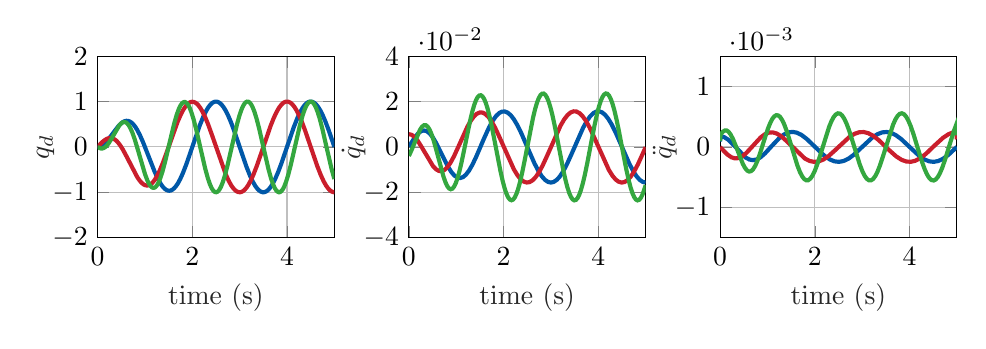
\begin{tikzpicture}

\begin{axis}[%
width=0.248\textwidth,
height=0.19\textwidth,
at={(0\textwidth,0\textwidth)},
scale only axis,
xmin=0,
xmax=5,
xlabel style={font=\color{white!15!black}},
xlabel={time (s)},
ymin=-2,
ymax=2,
ylabel style={font=\color{white!15!black}},
ylabel={$q_d$},
axis background/.style={fill=white},
xmajorgrids,
ymajorgrids,
ylabel style={yshift=-7.5pt}
]
\addplot [color=mycolor1, line width=1.5pt, forget plot]
  table[row sep=crcr]{%
0	0\\
0.035035035035035	0.00434065382436177\\
0.075075075075075	0.0197581919620422\\
0.115115115115115	0.0457558239801097\\
0.16016016016016	0.0864034559537759\\
0.215215215215215	0.149650792611576\\
0.29029029029029	0.251909193908196\\
0.435435435435435	0.452501851145034\\
0.49049049049049	0.511874966215594\\
0.535535535535535	0.547735702552471\\
0.575575575575575	0.567954316778994\\
0.61061061061061	0.575566933229249\\
0.645645645645645	0.573088771427073\\
0.68068068068068	0.560095653946306\\
0.715715715715715	0.536392535810649\\
0.755755755755755	0.496246230155413\\
0.795795795795796	0.442585433729294\\
0.840840840840841	0.367062318903137\\
0.895895895895896	0.255345156916537\\
0.960960960960961	0.101033017828754\\
1.05605605605606	-0.15149073785141\\
1.20620620620621	-0.550319348528045\\
1.27627627627628	-0.708764889034357\\
1.33133133133133	-0.811325353645943\\
1.37637637637638	-0.877772299605288\\
1.41641641641642	-0.922105295564261\\
1.45145145145145	-0.948751619733451\\
1.48648648648649	-0.963596043213059\\
1.51651651651652	-0.966718567647844\\
1.54654654654655	-0.960902245684151\\
1.57657657657658	-0.946171019746461\\
1.61161161161161	-0.91787491799227\\
1.65165165165165	-0.871308378489516\\
1.6966966966967	-0.801691383211872\\
1.74674674674675	-0.704652917692613\\
1.8018018018018	-0.576880303587744\\
1.87187187187187	-0.388564855615353\\
1.96696696696697	-0.103030019623617\\
2.15715715715716	0.472826180715402\\
2.22722722722723	0.653682856913231\\
2.28728728728729	0.783947303234589\\
2.33733733733734	0.871419229432251\\
2.38238238238238	0.931802645757189\\
2.42242242242242	0.969852863853533\\
2.45745745745746	0.990576346388929\\
2.48748748748749	0.99879275130267\\
2.51751751751752	0.998116211770342\\
2.54754754754755	0.988552949224476\\
2.58258258258258	0.966282396359661\\
2.61761761761762	0.932306066362887\\
2.65765765765766	0.87967759968175\\
2.7027027027027	0.803890788095862\\
2.75275275275275	0.700895927035849\\
2.81281281281281	0.554714287228555\\
2.88788788788789	0.344958268771602\\
3.003003003003	-0.00943386773232557\\
3.14314314314314	-0.43468926190012\\
3.21821821821822	-0.633097599682777\\
3.27827827827828	-0.767051472600784\\
3.32832832832833	-0.858054673447568\\
3.37337337337337	-0.921910196927753\\
3.41341341341341	-0.963228857786627\\
3.44844844844845	-0.986913031185399\\
3.48348348348348	-0.998653274574725\\
3.51351351351351	-0.999098293329462\\
3.54354354354354	-0.990657463060607\\
3.57857857857858	-0.96968362697153\\
3.61361361361361	-0.936974398085302\\
3.65365365365365	-0.885736697748763\\
3.6986986986987	-0.811413049476992\\
3.74874874874875	-0.709880810775015\\
3.80880880880881	-0.565174526154613\\
3.88388388388388	-0.356752674288018\\
3.99399399399399	-0.0188673044788441\\
4.14414414414414	0.437523008440333\\
4.21921921921922	0.635532084307429\\
4.27927927927928	0.769068005472834\\
4.32932932932933	0.859667579389312\\
4.37437437437437	0.923125598625732\\
4.41441441441441	0.964070346402118\\
4.44944944944945	0.987416293148271\\
4.48448448448448	0.998812274000765\\
4.51451451451451	0.998960559587034\\
4.54454454454454	0.990224253362287\\
4.57957957957958	0.968910783145196\\
4.61461461461461	0.935871305490616\\
4.65465465465465	0.884272782967919\\
4.6996996996997	0.809571163316425\\
4.74974974974975	0.707662478873392\\
4.80980980980981	0.562577458212637\\
4.88488488488488	0.353813119124604\\
5	8.88178419700125e-16\\
};
\addplot [color=mycolor2, line width=1.5pt, forget plot]
  table[row sep=crcr]{%
0	0\\
0.105105105105105	0.111779765028618\\
0.16016016016016	0.156980153648786\\
0.205205205205205	0.182511422079791\\
0.245245245245245	0.194668024428809\\
0.28028028028028	0.196227360736436\\
0.315315315315315	0.188769317384463\\
0.35035035035035	0.172022106528288\\
0.39039039039039	0.141487076700804\\
0.43043043043043	0.0991512285511922\\
0.475475475475475	0.0383838014112809\\
0.53053053053053	-0.0523767761630261\\
0.6006006006006	-0.18783198174113\\
0.840840840840841	-0.67188191620076\\
0.895895895895896	-0.752708585608064\\
0.940940940940941	-0.802692146771466\\
0.980980980980981	-0.833165316743078\\
1.01601601601602	-0.848168474733675\\
1.04604604604605	-0.851956160757179\\
1.07607607607608	-0.847156376186706\\
1.10610610610611	-0.833681829324347\\
1.14114114114114	-0.807033343602345\\
1.17617617617618	-0.768832354621136\\
1.21621621621622	-0.711564770634355\\
1.26126126126126	-0.63088812208567\\
1.31631631631632	-0.511373504538406\\
1.38138138138138	-0.345607907267669\\
1.46646646646647	-0.101148746562225\\
1.68668668668669	0.544000207265759\\
1.75175175175175	0.701576721741857\\
1.80680680680681	0.812683401978535\\
1.85685685685686	0.892797948975148\\
1.8968968968969	0.941073870130205\\
1.93193193193193	0.971074104183863\\
1.96696696696697	0.989241847338064\\
1.996996996997	0.995215537037103\\
2.02702702702703	0.992264006504053\\
2.05705705705706	0.980411255152744\\
2.09209209209209	0.95547795269928\\
2.12712712712713	0.918880529317171\\
2.16716716716717	0.863353759912902\\
2.21221221221221	0.7844957377737\\
2.26726726726727	0.666829747058395\\
2.33233233233233	0.502232140204002\\
2.41241241241241	0.271529840930044\\
2.7027027027027	-0.594554525970798\\
2.76776776776777	-0.745387426665372\\
2.82282282282282	-0.848990849411984\\
2.86786786786787	-0.915028120952007\\
2.90790790790791	-0.958401759441889\\
2.94294294294294	-0.983946634072939\\
2.97797797797798	-0.997582418387913\\
3.00800800800801	-0.999662561645784\\
3.03803803803804	-0.992851132434541\\
3.06806806806807	-0.977208771789291\\
3.1031031031031	-0.947988039568602\\
3.14314314314314	-0.900570748735437\\
3.18818818818819	-0.830261109785634\\
3.23823823823824	-0.732742817227718\\
3.29329329329329	-0.604697368948116\\
3.36336336336336	-0.41619419138787\\
3.45845845845846	-0.1301363223696\\
3.65365365365365	0.464187490802019\\
3.72372372372372	0.646393867785127\\
3.78378378378378	0.778035686293484\\
3.83383383383383	0.866810466126059\\
3.87887887887888	0.928474109611159\\
3.91891891891892	0.967732918025878\\
3.95395395395395	0.989555253702245\\
3.98398398398398	0.998734409694203\\
4.01401401401401	0.999030984234652\\
4.04404404404404	0.990442339782819\\
4.07907907907908	0.969298597922351\\
4.11411411411411	0.9364241544223\\
4.15415415415415	0.88500593597636\\
4.1991991991992	0.810493174479892\\
4.24924924924925	0.708772560434584\\
4.30930930930931	0.563876708920316\\
4.38438438438438	0.35528334276137\\
4.49449449449449	0.0172951932970005\\
4.63963963963964	-0.424754659261413\\
4.71471471471471	-0.624542944420901\\
4.77477477477477	-0.759946247977657\\
4.82482482482482	-0.852352489109542\\
4.86986986986987	-0.917592188634139\\
4.90990990990991	-0.96021468537402\\
4.94494494494494	-0.985079574464464\\
4.97997997997998	-0.99802277725853\\
5	-0.999999999998463\\
};
\addplot [color=mycolor3, line width=1.5pt, forget plot]
  table[row sep=crcr]{%
0	-0\\
0.04004004004004	-0.0253745100040801\\
0.07007007007007	-0.0347038050172159\\
0.1001001001001	-0.0347370008429007\\
0.13013013013013	-0.0250154145793022\\
0.16016016016016	-0.0054932552761473\\
0.195195195195195	0.0291506297466535\\
0.235235235235235	0.0827538361897568\\
0.285285285285285	0.16619460726963\\
0.46046046046046	0.476679866800188\\
0.5005005005005	0.520938149913881\\
0.53053053053053	0.541265433708041\\
0.555555555555555	0.548589477479468\\
0.58058058058058	0.546477201874926\\
0.605605605605605	0.534475742154076\\
0.63063063063063	0.512334606754345\\
0.66066066066066	0.472339342305941\\
0.695695695695695	0.407638563999009\\
0.735735735735735	0.311549516304309\\
0.785785785785786	0.162988678062016\\
0.850850850850851	-0.0635843329845418\\
1.001001001001	-0.598978538317431\\
1.05105105105105	-0.737906954073797\\
1.09109109109109	-0.822134211231833\\
1.12112112112112	-0.866793223366643\\
1.14614614614615	-0.890778796998402\\
1.17117117117117	-0.902132835176695\\
1.19119119119119	-0.901877449005232\\
1.21121121121121	-0.893224311557399\\
1.23623623623624	-0.870611388147704\\
1.26126126126126	-0.835084370833918\\
1.29129129129129	-0.775989311963286\\
1.32632632632633	-0.685754032567514\\
1.37137137137137	-0.539824281580024\\
1.42642642642643	-0.324964646431106\\
1.51151151151151	0.0524552962322513\\
1.61661661661662	0.51068147425186\\
1.67167167167167	0.710508039285358\\
1.71671671671672	0.839809432175977\\
1.75175175175175	0.914737029146651\\
1.78178178178178	0.959240382698092\\
1.80680680680681	0.981667705873682\\
1.82682682682683	0.989754892345688\\
1.84684684684685	0.988985560607153\\
1.86686686686687	0.979356598439477\\
1.89189189189189	0.954987957816951\\
1.91691691691692	0.917231880765766\\
1.94694694694695	0.854996252662267\\
1.98198198198198	0.760654843428203\\
2.02702702702703	0.609027332372115\\
2.08208208208208	0.386868838337833\\
2.16716716716717	-0.00235341420373558\\
2.27227227227227	-0.476740013733818\\
2.32732732732733	-0.686128439736638\\
2.37237237237237	-0.823872463922093\\
2.40740740740741	-0.905707232186816\\
2.43743743743744	-0.956312435519591\\
2.46246246246246	-0.983906356917698\\
2.48748748748749	-0.997827816311879\\
2.50750750750751	-0.99898359601381\\
2.52752752752753	-0.991250100548469\\
2.55255255255255	-0.969194596213682\\
2.57757757757758	-0.933668618821868\\
2.60760760760761	-0.873964134919092\\
2.64264264264264	-0.782315745941585\\
2.68768768768769	-0.633618002235095\\
2.74274274274274	-0.414005821608413\\
2.82282282282282	-0.0495061227704499\\
2.94294294294294	0.493844251052776\\
2.997997997998	0.700388748460756\\
3.04304304304304	0.835041499681637\\
3.07807807807808	0.914107856575382\\
3.10810810810811	0.962155969131873\\
3.13313313313313	0.98753105117545\\
3.15815815815816	0.99918833543435\\
3.17817817817818	0.998522048373447\\
3.1981981981982	0.988974942633285\\
3.22322322322322	0.964689233243766\\
3.24824824824825	0.927003009137534\\
3.27827827827828	0.864840650298925\\
3.31331331331331	0.770571225684974\\
3.35835835835836	0.619000071754701\\
3.41341341341341	0.396800981518273\\
3.4984984984985	0.00707559477390074\\
3.60860860860861	-0.489752472097759\\
3.66366366366366	-0.697029667042679\\
3.70870870870871	-0.832450937165657\\
3.74374374374374	-0.912197337060987\\
3.77377377377377	-0.960870579525157\\
3.7987987987988	-0.986786943557313\\
3.82382382382382	-0.998996023815813\\
3.84384384384384	-0.998773604988724\\
3.86386386386386	-0.989668255700024\\
3.88888888888889	-0.965925789545627\\
3.91391391391391	-0.928765818557316\\
3.94394394394394	-0.86720224931259\\
3.97897897897898	-0.77357123059458\\
4.02402402402402	-0.622699193733973\\
4.07907907907908	-0.401126949383538\\
4.16416416416416	-0.0117924918369763\\
4.27427427427427	0.485634538435109\\
4.32932932932933	0.693639713954403\\
4.37437437437437	0.82982807333996\\
4.40940940940941	0.910254465460059\\
4.43943943943944	0.959553358610013\\
4.46446446446446	0.986011765731368\\
4.48948948948949	0.998773659190625\\
4.50950950950951	0.998996087409785\\
4.52952952952953	0.990333607846368\\
4.55455455455455	0.967135952108439\\
4.57957957957958	0.930503983273733\\
4.60960960960961	0.869541525097858\\
4.64464464464464	0.776551901449321\\
4.68968968968969	0.626383213058514\\
4.74474474474474	0.405443448982906\\
4.82982982982983	0.0165091212806967\\
4.93993993993994	-0.481505636914043\\
4.99499499499499	-0.690234174264289\\
5	-0.707106781185458\\
};
\end{axis}

\begin{axis}[%
width=0.248\textwidth,
height=0.19\textwidth,
at={(0.326\textwidth,0\textwidth)},
scale only axis,
xmin=0,
xmax=5,
xlabel style={font=\color{white!15!black}},
xlabel={time (s)},
ymin=-0.04,
ymax=0.04,
ylabel style={font=\color{white!15!black}},
ylabel={$\dot{q}_d$},
axis background/.style={fill=white},
xmajorgrids,
ymajorgrids,
ylabel style={yshift=-7.5pt}
]
\addplot [color=mycolor1, line width=1.5pt, forget plot]
  table[row sep=crcr]{%
0	8.87958036743797e-05\\
0.02002002002002	0.000709205286566927\\
0.13013013013013	0.00431354598848444\\
0.2002002002002	0.00602568516306956\\
0.26026026026026	0.00693784257997976\\
0.32032032032032	0.00724490259747501\\
0.38038038038038	0.00690746540709775\\
0.44044044044044	0.00593471651671429\\
0.505505505505505	0.00422996742472659\\
0.575575575575575	0.00177973755126715\\
0.675675675675675	-0.00240049325539715\\
0.825825825825826	-0.00868090425285217\\
0.900900900900901	-0.0111658143824966\\
0.965965965965966	-0.0127084883031694\\
1.02602602602603	-0.0135312743668141\\
1.08608608608609	-0.0137280496105907\\
1.14614614614615	-0.0132868669616926\\
1.20620620620621	-0.0122291022584786\\
1.27127127127127	-0.0104477195110757\\
1.34134134134134	-0.0079022607533874\\
1.42642642642643	-0.00416316463676836\\
1.58658658658659	0.00368059325814496\\
1.69169169169169	0.00849151878580301\\
1.77177177177177	0.0115460906314997\\
1.84184184184184	0.0136041791124057\\
1.90690690690691	0.0149070651732561\\
1.96696696696697	0.0155416553906065\\
2.02702702702703	0.0156092580414757\\
2.08708708708709	0.0151099515853312\\
2.15215215215215	0.0139534009546507\\
2.21721721721722	0.01220713173322\\
2.29229229229229	0.00955913862891311\\
2.37737737737738	0.0059220893298475\\
2.5025025025025	-0.000112795085106754\\
2.65265265265265	-0.00724892771459817\\
2.73773773773774	-0.0106779731168718\\
2.80780780780781	-0.012940911941616\\
2.87287287287287	-0.0144843869759752\\
2.93793793793794	-0.0154244334183069\\
2.997997997998	-0.0157223717405444\\
3.05805805805806	-0.0154620801493941\\
3.12312312312312	-0.0145613972166379\\
3.18818818818819	-0.0130543490417994\\
3.25825825825826	-0.0108257718717653\\
3.33833833833834	-0.00764650755058938\\
3.43843843843844	-0.00302197280326677\\
3.67867867867868	0.00836963830915671\\
3.75875875875876	0.0114195404408468\\
3.82882882882883	0.0135039386224447\\
3.89389389389389	0.0148575485231452\\
3.95895895895896	0.0155925293693473\\
4.01901901901902	0.01569498110561\\
4.07907907907908	0.0152403197954696\\
4.14414414414414	0.0141382701809354\\
4.20920920920921	0.0124475408105065\\
4.27927927927928	0.0100496470917113\\
4.36436436436436	0.00649885919009208\\
4.47947947947948	0.00101291704575601\\
4.65465465465465	-0.00734219873027886\\
4.73973973973974	-0.0107537859157611\\
4.80980980980981	-0.0129989373491224\\
4.87487487487487	-0.0145238276366495\\
4.93993993993994	-0.0154439846312249\\
5	-0.0157230390570149\\
};
\addplot [color=mycolor2, line width=1.5pt, forget plot]
  table[row sep=crcr]{%
0	0.00564679810898916\\
0.06006006006006	0.00532698853810398\\
0.12012012012012	0.00439279220918198\\
0.185185185185185	0.00277385963725596\\
0.265265265265265	0.000135489686829082\\
0.51051051051051	-0.00846723701053786\\
0.575575575575575	-0.00988340148525158\\
0.635635635635635	-0.0105965516072484\\
0.695695695695695	-0.0106745781731705\\
0.755755755755755	-0.0100982489775987\\
0.815815815815816	-0.00889075730022348\\
0.880880880880881	-0.00694328214617457\\
0.950950950950951	-0.00424090998455195\\
1.04604604604605	8.04961082803146e-05\\
1.23623623623624	0.0088695371597316\\
1.31131131131131	0.0116449451465765\\
1.37637637637638	0.0134795293660801\\
1.43643643643644	0.0146177117690955\\
1.4964964964965	0.0151759125248292\\
1.55655655655656	0.0151350477011531\\
1.61661661661662	0.014501321548952\\
1.68168168168168	0.0131809237407268\\
1.74674674674675	0.0112662147885771\\
1.82182182182182	0.00843852080878538\\
1.91191191191191	0.00440679951085077\\
2.21721721721722	-0.00986682322024279\\
2.29229229229229	-0.0124599594878632\\
2.36236236236236	-0.0142550761271227\\
2.42742742742743	-0.0153034838841499\\
2.48748748748749	-0.015703599140477\\
2.54754754754755	-0.0155443311943841\\
2.61261261261261	-0.0147481695643945\\
2.67767767767768	-0.0133367782902223\\
2.74774774774775	-0.0111971986946333\\
2.82282282282282	-0.00830788352575418\\
2.91791791791792	-0.00401063830401949\\
3.2032032032032	0.00936909186312107\\
3.27827827827828	0.0120603023051942\\
3.34834834834835	0.0139720380102135\\
3.41341341341341	0.0151448717266796\\
3.47847847847848	0.0156870991330482\\
3.53853853853854	0.0156079352179992\\
3.6036036036036	0.0148975351922962\\
3.66866866866867	0.0135668386233387\\
3.73873873873874	0.0115041615729501\\
3.81381381381381	0.00868122055632714\\
3.9039039039039	0.00467492977406625\\
4.22422422422422	-0.0101821280708343\\
4.2992992992993	-0.012699830891715\\
4.36436436436436	-0.0143170802219998\\
4.42942942942943	-0.015338204655519\\
4.49449449449449	-0.0157206873108446\\
4.55455455455455	-0.0154926801893511\\
4.61961961961962	-0.0146258182674659\\
4.68468468468468	-0.0131499764352121\\
4.75475475475475	-0.010950560202887\\
4.83483483483483	-0.00779720158670827\\
4.93493493493493	-0.00319157963644301\\
5	-0.000123614618962264\\
};
\addplot [color=mycolor3, line width=1.5pt, forget plot]
  table[row sep=crcr]{%
0	-0.00389809489151549\\
0.015015015015015	-0.00339743312423035\\
0.07007007007007	-0.000798049903772302\\
0.235235235235235	0.0075242798095152\\
0.28028028028028	0.00891341777412347\\
0.32032032032032	0.00954886517354314\\
0.36036036036036	0.00954325489899865\\
0.4004004004004	0.00886314945613709\\
0.44044044044044	0.00751665139384627\\
0.48048048048048	0.00555306089437746\\
0.525525525525525	0.00271691090566417\\
0.58058058058058	-0.00140005508322449\\
0.73073073073073	-0.013047466318822\\
0.775775775775776	-0.015698623308781\\
0.815815815815816	-0.0174204385094043\\
0.850850850850851	-0.018349425338215\\
0.885885885885886	-0.0186874682652869\\
0.920920920920921	-0.0184077208485345\\
0.955955955955956	-0.0175061165448778\\
0.990990990990991	-0.0160013355837796\\
1.02602602602603	-0.0139339061890249\\
1.06606606606607	-0.0109608486185069\\
1.11111111111111	-0.00698189751919642\\
1.17117117117117	-0.000980351284410652\\
1.2962962962963	0.0117619630177312\\
1.34134134134134	0.0156578685080238\\
1.38138138138138	0.0185348794184224\\
1.41641641641642	0.0205023889787048\\
1.45145145145145	0.0218918110674409\\
1.48648648648649	0.0226596686069893\\
1.52152152152152	0.0227814208285331\\
1.55655655655656	0.0222519519447575\\
1.59159159159159	0.0210854742708797\\
1.62662662662663	0.0193148692864513\\
1.66166166166166	0.0169905040707912\\
1.7017017017017	0.01374157480143\\
1.74674674674675	0.00947671453637522\\
1.80680680680681	0.00312319721480137\\
1.93693693693694	-0.0108766793959374\\
1.98198198198198	-0.0150397082531191\\
2.02202202202202	-0.0181763491351035\\
2.06206206206206	-0.0206640010925963\\
2.0970970970971	-0.0222375006152946\\
2.13213213213213	-0.0232022701913621\\
2.16716716716717	-0.0235320248963236\\
2.2022022022022	-0.0232179498720821\\
2.23723723723724	-0.0222688850183692\\
2.27227227227227	-0.0207110348795023\\
2.30730730730731	-0.0185872130621734\\
2.34734734734735	-0.0155422967374443\\
2.39239239239239	-0.0114608139600945\\
2.44744744744745	-0.00579145047336116\\
2.62262262262262	0.0128741520625955\\
2.66766766766767	0.0167484861142819\\
2.70770770770771	0.0195655424407741\\
2.74274274274274	0.0214633257479662\\
2.77777777777778	0.0227771606090883\\
2.81281281281281	0.0234713332423633\\
2.84784784784785	0.0235269892600414\\
2.88288288288288	0.0229426428669539\\
2.91791791791792	0.0217342145445576\\
2.95295295295295	0.0199345961159061\\
2.99299299299299	0.0172174864691881\\
3.03303303303303	0.0138891400020897\\
3.07807807807808	0.00956198015215293\\
3.13813813813814	0.00316121176298179\\
3.26326326326326	-0.0103680819172496\\
3.30830830830831	-0.0145980008421667\\
3.34834834834835	-0.0178130752410732\\
3.38838838838839	-0.0203958438019916\\
3.42342342342342	-0.0220643905498283\\
3.45845845845846	-0.0231328750670352\\
3.49349349349349	-0.0235722399853806\\
3.52852852852853	-0.0233705372810213\\
3.56356356356356	-0.0225332531602396\\
3.5985985985986	-0.0210831588311615\\
3.63363363363363	-0.0190596912137808\\
3.67367367367367	-0.0161163193506209\\
3.71871871871872	-0.0121272464772959\\
3.76876876876877	-0.00706512219780375\\
3.85385385385385	0.00227697060687326\\
3.92392392392392	0.00976466521871266\\
3.97397397397397	0.0145105874986564\\
4.01401401401401	0.0177400615962862\\
4.05405405405405	0.0203398300274422\\
4.08908908908909	0.0220249114397006\\
4.12412412412412	0.0231110093381206\\
4.15915915915916	0.0235685865111357\\
4.19419419419419	0.0233851988235765\\
4.22922922922923	0.0225658336438439\\
4.26426426426426	0.0211327742088825\\
4.2992992992993	0.0191249936155176\\
4.33933933933934	0.0161973536236735\\
4.38438438438438	0.0122225178974782\\
4.43443443443443	0.00717117600018735\\
4.51951951951952	-0.00216622237303721\\
4.59459459459459	-0.0101679498965721\\
4.64464464464464	-0.0148587632807544\\
4.68468468468468	-0.0180300857626401\\
4.72472472472472	-0.0205614078968743\\
4.75975975975976	-0.0221800565341406\\
4.79479479479479	-0.0231955024176012\\
4.82982982982983	-0.0235801297586606\\
4.86486486486486	-0.0233234783373355\\
4.8998998998999	-0.0224325279755435\\
4.93493493493493	-0.0209315087157567\\
4.96996996996997	-0.0188612418674117\\
5	-0.0168726069211687\\
};
\end{axis}

\begin{axis}[%
width=0.248\textwidth,
height=0.19\textwidth,
at={(0.652\textwidth,0\textwidth)},
scale only axis,
xmin=0,
xmax=5,
xlabel style={font=\color{white!15!black}},
xlabel={time (s)},
ymin=-0.0015,
ymax=0.0015,
ylabel style={font=\color{white!15!black}},
ylabel={$\ddot{q}_d$},
axis background/.style={fill=white},
xmajorgrids,
ymajorgrids,
ylabel style={yshift=-7.5pt}
]
\addplot [color=mycolor1, line width=1.5pt, forget plot]
  table[row sep=crcr]{%
0	8.87694027520425e-05\\
0.01001001001001	0.00017735405761421\\
0.0850850850850851	0.000162509474272987\\
0.165165165165165	0.000122898614725919\\
0.26026026026026	5.16757315711658e-05\\
0.54054054054054	-0.000175647586806882\\
0.62062062062062	-0.000209228561418584\\
0.695695695695695	-0.000219191647969907\\
0.77077077077077	-0.000207634659953548\\
0.850850850850851	-0.000173432942190743\\
0.945945945945946	-0.000109438530278894\\
1.09109109109109	1.47030712716045e-05\\
1.25125125125125	0.000146365773517232\\
1.35135135135135	0.000206488771483215\\
1.44144144144144	0.000238914807979107\\
1.53153153153153	0.00024847529676908\\
1.62162162162162	0.00023528471028289\\
1.71671671671672	0.000199003383504426\\
1.82682682682683	0.000134003966592466\\
1.98198198198198	1.7529457647214e-05\\
2.2022022022022	-0.000145877176117359\\
2.31731731731732	-0.000207451177407059\\
2.41741741741742	-0.000239040821556458\\
2.51251251251251	-0.000247198882016519\\
2.60760760760761	-0.000233389446901988\\
2.70770770770771	-0.000196548359442161\\
2.82282282282282	-0.000130680489912827\\
2.97797797797798	-1.7115820638125e-05\\
3.20820820820821	0.000150415316355179\\
3.32332332332332	0.000210101746477953\\
3.42342342342342	0.000240095502739734\\
3.51851851851852	0.000246796427739504\\
3.61361361361361	0.000231633689296018\\
3.71371371371371	0.000193556575021958\\
3.82882882882883	0.000126624312621004\\
3.98898898898899	8.54996996313417e-06\\
4.2042042042042	-0.000147937549992427\\
4.31931931931932	-0.000208445907700749\\
4.41941941941942	-0.000239334742854425\\
4.51451451451451	-0.000246956993382064\\
4.60960960960961	-0.000232701386970291\\
4.70970970970971	-0.00019547544774845\\
4.82482482482482	-0.000129284919124117\\
4.98498498498498	-1.16570204786726e-05\\
5	-1.94359748117989e-06\\
};
\addplot [color=mycolor2, line width=1.5pt, forget plot]
  table[row sep=crcr]{%
0	-2.23556281042647e-06\\
0.03003003003003	-2.67367789250628e-05\\
0.155155155155155	-0.000126683269910721\\
0.24024024024024	-0.000172055232029678\\
0.315315315315315	-0.000189961457533805\\
0.39039039039039	-0.00018488709411546\\
0.465465465465465	-0.000157537612884617\\
0.55055055055055	-0.000103813924305918\\
0.665665665665665	-6.56691347611371e-06\\
0.855855855855856	0.000155581983405817\\
0.945945945945946	0.00020882745164208\\
1.03103103103103	0.000236407125877136\\
1.11111111111111	0.000240171194534788\\
1.1961961961962	0.000221156105233433\\
1.28628628628629	0.000178417908525574\\
1.3963963963964	0.000102764156034496\\
1.79179179179179	-0.000192856850054213\\
1.89189189189189	-0.000232514765528435\\
1.98698698698699	-0.000247807965711999\\
2.08208208208208	-0.000240350679932888\\
2.18218218218218	-0.000209103818113121\\
2.29229229229229	-0.00015107830541794\\
2.43243243243243	-5.25983850856448e-05\\
2.72772772772773	0.000162119684500084\\
2.83783783783784	0.000215825326704611\\
2.93793793793794	0.000242544962231861\\
3.03303303303303	0.000245898657150079\\
3.12812812812813	0.000227466059277148\\
3.23323323323323	0.000183774243206258\\
3.35335335335335	0.000109909045222345\\
3.54854854854855	-3.75584871763479e-05\\
3.71871871871872	-0.000156812066847145\\
3.83383383383383	-0.000214287686508996\\
3.93393393393393	-0.000241908317786255\\
4.02902902902903	-0.000246186653521718\\
4.12412412412412	-0.00022865537912331\\
4.22922922922923	-0.000185833258132817\\
4.34934934934935	-0.000112682802556385\\
4.53453453453453	2.67685056707379e-05\\
4.70970970970971	0.000151340972588621\\
4.82482482482482	0.000210713431763487\\
4.92492492492492	0.000240369797759321\\
4.98998998998999	0.000247091727711535\\
5	0.000123599338309077\\
};
\addplot [color=mycolor3, line width=1.5pt, forget plot]
  table[row sep=crcr]{%
0	9.75515083148082e-05\\
0.01001001001001	0.000201555129485165\\
0.055055055055055	0.000248489426118326\\
0.1001001001001	0.000271819748162372\\
0.14014014014014	0.000270938386123021\\
0.18018018018018	0.000249519009343224\\
0.225225225225225	0.000202382486667929\\
0.275275275275275	0.00012565322232394\\
0.335335335335335	9.83810009902442e-06\\
0.48048048048048	-0.000280701781798065\\
0.53053053053053	-0.000352226610364603\\
0.575575575575575	-0.000393140949621618\\
0.615615615615615	-0.000407846833930137\\
0.655655655655655	-0.000400851594310581\\
0.695695695695695	-0.000372140551254674\\
0.74074074074074	-0.000315389469616179\\
0.785785785785786	-0.000235998174186847\\
0.840840840840841	-0.000115347468549132\\
0.930930930930931	0.000109955420625418\\
1.01101101101101	0.000301129490159369\\
1.06106106106106	0.000399325858168709\\
1.10610610610611	0.000466410747031354\\
1.14614614614615	0.00050583374910218\\
1.18618618618619	0.000524395837762093\\
1.22622622622623	0.000521305492251933\\
1.26626626626627	0.0004967248207981\\
1.31131131131131	0.000444760976283654\\
1.35635635635636	0.000369789370585849\\
1.40640640640641	0.000264345934837706\\
1.47147147147147	0.000103311506659765\\
1.63163163163163	-0.00030510631456071\\
1.68668668668669	-0.000415657817936399\\
1.73173173173173	-0.000484774468885618\\
1.77677677677678	-0.000531244361556382\\
1.82182182182182	-0.000553007311978604\\
1.86186186186186	-0.000550860258392127\\
1.90690690690691	-0.000524471199531362\\
1.95195195195195	-0.000473999655953072\\
1.996996996997	-0.000401850505259205\\
2.04704704704705	-0.000300388000582075\\
2.11211211211211	-0.000144340246710506\\
2.3023023023023	0.00033071872456425\\
2.35235235235235	0.000426249156026515\\
2.3973973973974	0.000492064536011583\\
2.44244244244244	0.000535703046027791\\
2.48748748748749	0.000555221903511871\\
2.53253253253253	0.000549761694288442\\
2.57757757757758	0.000519583311266558\\
2.62262262262262	0.000466055209937366\\
2.67267267267267	0.000382162739451353\\
2.72772772772773	0.000265648807288521\\
2.7977977977978	9.28088762002233e-05\\
2.94794794794795	-0.000285968168891593\\
3.003003003003	-0.000398783856231155\\
3.05305305305305	-0.000478341638006974\\
3.0980980980981	-0.000527390721217991\\
3.14314314314314	-0.000552763095249986\\
3.18818818818819	-0.000553320604391061\\
3.23323323323323	-0.000529038851106556\\
3.27827827827828	-0.000481008296750574\\
3.32332332332332	-0.000411385331102743\\
3.37337337337337	-0.000312532587591896\\
3.43343343343343	-0.000171619891333741\\
3.65365365365365	0.000368433668802126\\
3.7037037037037	0.000455591101735209\\
3.74874874874875	0.000512573982865305\\
3.79379379379379	0.000546547629265426\\
3.83883883883884	0.000555986994196012\\
3.88388388388388	0.000540468358728674\\
3.92892892892893	0.000500688353204382\\
3.97397397397397	0.000438432686718393\\
4.02402402402402	0.000346329199443218\\
4.08408408408408	0.000211019434059878\\
4.17417417417417	-1.96723805281351e-05\\
4.26926926926927	-0.000258556335277049\\
4.32432432432432	-0.00037622908500623\\
4.37437437437437	-0.000461528886519957\\
4.41941941941942	-0.000516555514463946\\
4.46446446446446	-0.000548394212072978\\
4.50950950950951	-0.000555615755507333\\
4.55455455455455	-0.00053789597317877\\
4.5995995995996	-0.000496030297673755\\
4.64464464464464	-0.000431898059166436\\
4.69469469469469	-0.0003380567608815\\
4.75475475475475	-0.000201272972605082\\
4.84984984984985	4.32445897455835e-05\\
4.93993993993994	0.000267800966806675\\
4.98998998998999	0.00037429272768108\\
5	0.000191971883321429\\
};
\end{axis}
\end{tikzpicture}%
  \fi
  \vspace{-3mm}
  \caption{The time evolution of the predefined geometric strain parameters of the Piece-wise Constant curvature model $\q_d \to  (\varepsilon, \, \kappa_x,\,\kappa_y)^\top$ and their corresponding time-derivatives $\dq_d$ and $\ddq_d$, given by the (constant) elongation $\varepsilon$ \data{Matlab1}, and the (constant) curvatures $\kappa_x$ \data{Matlab2} and $\kappa_y$ \data{Matlab3}.}
  \label{fig:C2:EX1:strain_ref}
\end{figure}

\end{example}

\afterpage{
\begin{figure}[!t]
  \vspace{-3mm}
  %\centering
  \ifx\printFigures\undefined
  \else
  % This file was created by matlab2tikz.
%
\definecolor{mycolor1}{rgb}{0.89290,0.89290,0.89290}%
\definecolor{mycolor2}{rgb}{0.88840,0.88720,0.89330}%
\definecolor{mycolor3}{rgb}{0.88390,0.88140,0.89360}%
\definecolor{mycolor4}{rgb}{0.87940,0.87570,0.89400}%
\definecolor{mycolor5}{rgb}{0.87490,0.87000,0.89440}%
\definecolor{mycolor6}{rgb}{0.87040,0.86420,0.89470}%
\definecolor{mycolor7}{rgb}{0.86590,0.85850,0.89510}%
\definecolor{mycolor8}{rgb}{0.86140,0.85280,0.89550}%
\definecolor{mycolor9}{rgb}{0.85690,0.84700,0.89590}%
\definecolor{mycolor10}{rgb}{0.85240,0.84130,0.89620}%
\definecolor{mycolor11}{rgb}{0.84790,0.83560,0.89660}%
\definecolor{mycolor12}{rgb}{0.84340,0.82990,0.89700}%
\definecolor{mycolor13}{rgb}{0.83890,0.82410,0.89730}%
\definecolor{mycolor14}{rgb}{0.83440,0.81840,0.89770}%
\definecolor{mycolor15}{rgb}{0.82990,0.81270,0.89810}%
\definecolor{mycolor16}{rgb}{0.82530,0.80690,0.89840}%
\definecolor{mycolor17}{rgb}{0.82080,0.80120,0.89880}%
\definecolor{mycolor18}{rgb}{0.81630,0.79550,0.89920}%
\definecolor{mycolor19}{rgb}{0.81180,0.78970,0.89950}%
\definecolor{mycolor20}{rgb}{0.80730,0.78400,0.89990}%
\definecolor{mycolor21}{rgb}{0.80280,0.77830,0.90030}%
\definecolor{mycolor22}{rgb}{0.79830,0.77250,0.90060}%
\definecolor{mycolor23}{rgb}{0.79380,0.76680,0.90100}%
\definecolor{mycolor24}{rgb}{0.78930,0.76110,0.90140}%
\definecolor{mycolor25}{rgb}{0.78480,0.75530,0.90180}%
\definecolor{mycolor26}{rgb}{0.78030,0.74960,0.90210}%
\definecolor{mycolor27}{rgb}{0.77580,0.74390,0.90250}%
\definecolor{mycolor28}{rgb}{0.77130,0.73820,0.90290}%
\definecolor{mycolor29}{rgb}{0.76680,0.73240,0.90320}%
\definecolor{mycolor30}{rgb}{0.76230,0.72670,0.90360}%
\definecolor{mycolor31}{rgb}{0.75780,0.72100,0.90400}%
\definecolor{mycolor32}{rgb}{0.75330,0.71520,0.90430}%
\definecolor{mycolor33}{rgb}{0.74880,0.70950,0.90470}%
\definecolor{mycolor34}{rgb}{0.74430,0.70380,0.90510}%
\definecolor{mycolor35}{rgb}{0.73980,0.69800,0.90540}%
\definecolor{mycolor36}{rgb}{0.73530,0.69230,0.90580}%
\definecolor{mycolor37}{rgb}{0.73080,0.68660,0.90620}%
\definecolor{mycolor38}{rgb}{0.72630,0.68080,0.90650}%
\definecolor{mycolor39}{rgb}{0.72180,0.67510,0.90690}%
\definecolor{mycolor40}{rgb}{0.71730,0.66940,0.90730}%
\definecolor{mycolor41}{rgb}{0.71280,0.66360,0.90770}%
\definecolor{mycolor42}{rgb}{0.70830,0.65790,0.90800}%
\definecolor{mycolor43}{rgb}{0.70380,0.65220,0.90840}%
\definecolor{mycolor44}{rgb}{0.69930,0.64640,0.90880}%
\definecolor{mycolor45}{rgb}{0.69470,0.64070,0.90910}%
\definecolor{mycolor46}{rgb}{0.69020,0.63500,0.90950}%
\definecolor{mycolor47}{rgb}{0.68570,0.62930,0.90990}%
\definecolor{mycolor48}{rgb}{0.68120,0.62350,0.91020}%
\definecolor{mycolor49}{rgb}{0.67670,0.61780,0.91060}%
\definecolor{mycolor50}{rgb}{0.67220,0.61210,0.91100}%
\definecolor{mycolor51}{rgb}{0.66770,0.60630,0.91130}%
\definecolor{mycolor52}{rgb}{0.66320,0.60060,0.91170}%
\definecolor{mycolor53}{rgb}{0.65870,0.59490,0.91210}%
\definecolor{mycolor54}{rgb}{0.65420,0.58910,0.91240}%
\definecolor{mycolor55}{rgb}{0.64970,0.58340,0.91280}%
\definecolor{mycolor56}{rgb}{0.64520,0.57770,0.91320}%
\definecolor{mycolor57}{rgb}{0.64070,0.57190,0.91360}%
\definecolor{mycolor58}{rgb}{0.63620,0.56620,0.91390}%
\definecolor{mycolor59}{rgb}{0.63170,0.56050,0.91430}%
\definecolor{mycolor60}{rgb}{0.62720,0.55470,0.91470}%
\definecolor{mycolor61}{rgb}{0.62270,0.54900,0.91500}%
\definecolor{mycolor62}{rgb}{0.61820,0.54330,0.91540}%
\definecolor{mycolor63}{rgb}{0.61370,0.53760,0.91580}%
\definecolor{mycolor64}{rgb}{0.60920,0.53180,0.91610}%
\definecolor{mycolor65}{rgb}{0.60470,0.52610,0.91650}%
\definecolor{mycolor66}{rgb}{0.60020,0.52040,0.91690}%
\definecolor{mycolor67}{rgb}{0.59570,0.51460,0.91720}%
\definecolor{mycolor68}{rgb}{0.59120,0.50890,0.91760}%
\definecolor{mycolor69}{rgb}{0.58670,0.50320,0.91800}%
\definecolor{mycolor70}{rgb}{0.58220,0.49740,0.91830}%
\definecolor{mycolor71}{rgb}{0.57770,0.49170,0.91870}%
\definecolor{mycolor72}{rgb}{0.57320,0.48600,0.91910}%
\definecolor{mycolor73}{rgb}{0.56870,0.48020,0.91950}%
\definecolor{mycolor74}{rgb}{0.56410,0.47450,0.91980}%
\definecolor{mycolor75}{rgb}{0.55960,0.46880,0.92020}%
\definecolor{mycolor76}{rgb}{0.55510,0.46300,0.92060}%
\definecolor{mycolor77}{rgb}{0.55060,0.45730,0.92090}%
\definecolor{mycolor78}{rgb}{0.54610,0.45160,0.92130}%
\definecolor{mycolor79}{rgb}{0.54160,0.44580,0.92170}%
\definecolor{mycolor80}{rgb}{0.53710,0.44010,0.92200}%
\definecolor{mycolor81}{rgb}{0.53260,0.43440,0.92240}%
\definecolor{mycolor82}{rgb}{0.52810,0.42870,0.92280}%
\definecolor{mycolor83}{rgb}{0.52360,0.42290,0.92310}%
\definecolor{mycolor84}{rgb}{0.51910,0.41720,0.92350}%
\definecolor{mycolor85}{rgb}{0.51460,0.41150,0.92390}%
\definecolor{mycolor86}{rgb}{0.51010,0.40570,0.92420}%
\definecolor{mycolor87}{rgb}{0.50560,0.40000,0.92460}%
\definecolor{mycolor88}{rgb}{0.50110,0.39430,0.92500}%
\definecolor{mycolor89}{rgb}{0.49660,0.38850,0.92540}%
\definecolor{mycolor90}{rgb}{0.49210,0.38280,0.92570}%
\definecolor{mycolor91}{rgb}{0.48760,0.37710,0.92610}%
\definecolor{mycolor92}{rgb}{0.48310,0.37130,0.92650}%
\definecolor{mycolor93}{rgb}{0.47860,0.36560,0.92680}%
\definecolor{mycolor94}{rgb}{0.47410,0.35990,0.92720}%
\definecolor{mycolor95}{rgb}{0.46960,0.35410,0.92760}%
\definecolor{mycolor96}{rgb}{0.46510,0.34840,0.92790}%
\definecolor{mycolor97}{rgb}{0.46060,0.34270,0.92830}%
\definecolor{mycolor98}{rgb}{0.45610,0.33700,0.92870}%
\definecolor{mycolor99}{rgb}{0.45160,0.33120,0.92900}%
\definecolor{mycolor100}{rgb}{0.44710,0.32550,0.92940}%
\definecolor{mycolor101}{rgb}{0.00000,0.34510,0.65882}%
\definecolor{mycolor102}{rgb}{0.79216,0.11765,0.17255}%
\definecolor{mycolor103}{rgb}{0.20392,0.65490,0.24706}%
%
\begin{tikzpicture}

\begin{axis}[%
width=0.288\textwidth,
height=0.3\textwidth,
at={(0\textwidth,0\textwidth)},
scale only axis,
point meta min=0,
point meta max=6,
xmin=-1,
xmax=1,
xlabel style={font=\color{white!15!black}},
xlabel={$X$ (m)},
ymin=-1,
ymax=1,
ylabel style={font=\color{white!15!black}},
ylabel={$Y$ (m)},
axis background/.style={fill=white},
xmajorgrids,
ymajorgrids,
colorbar style={width=6,xshift=-7.5pt},
colormap={mymap}{[1pt] rgb(0pt)=(0.8929,0.8929,0.8929); rgb(1pt)=(0.8884,0.8872,0.8933); rgb(2pt)=(0.8839,0.8814,0.8936); rgb(4pt)=(0.8749,0.87,0.8944); rgb(5pt)=(0.8704,0.8642,0.8947); rgb(7pt)=(0.8614,0.8528,0.8955); rgb(8pt)=(0.8569,0.847,0.8959); rgb(9pt)=(0.8524,0.8413,0.8962); rgb(11pt)=(0.8434,0.8299,0.897); rgb(12pt)=(0.8389,0.8241,0.8973); rgb(14pt)=(0.8299,0.8127,0.8981); rgb(15pt)=(0.8253,0.8069,0.8984); rgb(17pt)=(0.8163,0.7955,0.8992); rgb(18pt)=(0.8118,0.7897,0.8995); rgb(20pt)=(0.8028,0.7783,0.9003); rgb(21pt)=(0.7983,0.7725,0.9006); rgb(23pt)=(0.7893,0.7611,0.9014); rgb(24pt)=(0.7848,0.7553,0.9018); rgb(25pt)=(0.7803,0.7496,0.9021); rgb(27pt)=(0.7713,0.7382,0.9029); rgb(28pt)=(0.7668,0.7324,0.9032); rgb(30pt)=(0.7578,0.721,0.904); rgb(31pt)=(0.7533,0.7152,0.9043); rgb(33pt)=(0.7443,0.7038,0.9051); rgb(34pt)=(0.7398,0.698,0.9054); rgb(36pt)=(0.7308,0.6866,0.9062); rgb(37pt)=(0.7263,0.6808,0.9065); rgb(39pt)=(0.7173,0.6694,0.9073); rgb(40pt)=(0.7128,0.6636,0.9077); rgb(41pt)=(0.7083,0.6579,0.908); rgb(42pt)=(0.7038,0.6522,0.9084); rgb(43pt)=(0.6993,0.6464,0.9088); rgb(44pt)=(0.6947,0.6407,0.9091); rgb(46pt)=(0.6857,0.6293,0.9099); rgb(47pt)=(0.6812,0.6235,0.9102); rgb(49pt)=(0.6722,0.6121,0.911); rgb(50pt)=(0.6677,0.6063,0.9113); rgb(52pt)=(0.6587,0.5949,0.9121); rgb(53pt)=(0.6542,0.5891,0.9124); rgb(55pt)=(0.6452,0.5777,0.9132); rgb(56pt)=(0.6407,0.5719,0.9136); rgb(57pt)=(0.6362,0.5662,0.9139); rgb(58pt)=(0.6317,0.5605,0.9143); rgb(59pt)=(0.6272,0.5547,0.9147); rgb(60pt)=(0.6227,0.549,0.915); rgb(62pt)=(0.6137,0.5376,0.9158); rgb(63pt)=(0.6092,0.5318,0.9161); rgb(65pt)=(0.6002,0.5204,0.9169); rgb(66pt)=(0.5957,0.5146,0.9172); rgb(68pt)=(0.5867,0.5032,0.918); rgb(69pt)=(0.5822,0.4974,0.9183); rgb(71pt)=(0.5732,0.486,0.9191); rgb(72pt)=(0.5687,0.4802,0.9195); rgb(73pt)=(0.5641,0.4745,0.9198); rgb(74pt)=(0.5596,0.4688,0.9202); rgb(75pt)=(0.5551,0.463,0.9206); rgb(76pt)=(0.5506,0.4573,0.9209); rgb(77pt)=(0.5461,0.4516,0.9213); rgb(78pt)=(0.5416,0.4458,0.9217); rgb(79pt)=(0.5371,0.4401,0.922); rgb(81pt)=(0.5281,0.4287,0.9228); rgb(82pt)=(0.5236,0.4229,0.9231); rgb(84pt)=(0.5146,0.4115,0.9239); rgb(85pt)=(0.5101,0.4057,0.9242); rgb(87pt)=(0.5011,0.3943,0.925); rgb(88pt)=(0.4966,0.3885,0.9254); rgb(89pt)=(0.4921,0.3828,0.9257); rgb(90pt)=(0.4876,0.3771,0.9261); rgb(91pt)=(0.4831,0.3713,0.9265); rgb(92pt)=(0.4786,0.3656,0.9268); rgb(93pt)=(0.4741,0.3599,0.9272); rgb(94pt)=(0.4696,0.3541,0.9276); rgb(95pt)=(0.4651,0.3484,0.9279); rgb(97pt)=(0.4561,0.337,0.9287); rgb(98pt)=(0.4516,0.3312,0.929); rgb(99pt)=(0.4471,0.3255,0.9294)},
colorbar
]
\addplot [color=mycolor1, line width=1.5pt, forget plot]
  table[row sep=crcr]{%
-4.90148069701157e-13	4.90148069701157e-13\\
-7.88107637255809e-05	0.000553125875846971\\
};
\addplot [color=mycolor2, line width=1.5pt, forget plot]
  table[row sep=crcr]{%
-7.88107637255805e-05	0.00055312587584697\\
-0.00152251679494098	0.0049436537853027\\
};
\addplot [color=mycolor3, line width=1.5pt, forget plot]
  table[row sep=crcr]{%
-0.00152251679494098	0.0049436537853027\\
-0.00787897041630117	0.0160643200797801\\
};
\addplot [color=mycolor4, line width=1.5pt, forget plot]
  table[row sep=crcr]{%
-0.00787897041630117	0.0160643200797801\\
-0.0240819114229362	0.0342203870599918\\
};
\addplot [color=mycolor5, line width=1.5pt, forget plot]
  table[row sep=crcr]{%
-0.0240819114229362	0.0342203870599918\\
-0.0439066143470563	0.04972968764855\\
-0.0549291537951963	0.0565951638082979\\
};
\addplot [color=mycolor6, line width=1.5pt, forget plot]
  table[row sep=crcr]{%
-0.0549291537951963	0.0565951638082979\\
-0.0818483861230205	0.0697828529507438\\
-0.10346214702107	0.0775316923087539\\
};

\addplot[area legend, draw=none, fill=mycolor6, forget plot]
table[row sep=crcr] {%
x	y\\
-0.085169602328192	0.034242717861915\\
-0.10346214702107	0.0775316923087539\\
-0.0690491494155618	0.109536349716752\\
-0.235226002767034	0.105742484905857\\
}--cycle;
\addplot [color=mycolor7, line width=1.5pt, forget plot]
  table[row sep=crcr]{%
-0.10346214702107	0.0775316923087539\\
-0.141210938516005	0.0863359599060765\\
-0.169646879099566	0.0895881214185072\\
};
\addplot [color=mycolor8, line width=1.5pt, forget plot]
  table[row sep=crcr]{%
-0.169646879099566	0.0895881214185072\\
-0.208322128327543	0.0898617174104523\\
-0.249690027242874	0.085142046238163\\
};
\addplot [color=mycolor9, line width=1.5pt, forget plot]
  table[row sep=crcr]{%
-0.249690027242874	0.085142046238163\\
-0.292712580905681	0.0747443599796589\\
-0.327514447856391	0.0620077575291899\\
-0.336181345109123	0.0581889689879663\\
};
\addplot [color=mycolor10, line width=1.5pt, forget plot]
  table[row sep=crcr]{%
-0.336181345109123	0.0581889689879663\\
-0.370385993231795	0.0403435425483828\\
-0.403311036652028	0.0184039714785172\\
-0.419067849983946	0.00593155832663744\\
};
\addplot [color=mycolor11, line width=1.5pt, forget plot]
  table[row sep=crcr]{%
-0.419067849983946	0.00593155832663744\\
-0.448723581236193	-0.0218887827678687\\
-0.475327597127939	-0.0532852960219785\\
-0.487280330891912	-0.0702015200303958\\
};
\addplot [color=mycolor12, line width=1.5pt, forget plot]
  table[row sep=crcr]{%
-0.487280330891912	-0.0702015200303958\\
-0.508110849209801	-0.106165473966\\
-0.524396277107342	-0.144494856080128\\
-0.530689055157139	-0.164347646914564\\
};

\addplot[area legend, draw=none, fill=mycolor12, forget plot]
table[row sep=crcr] {%
x	y\\
-0.487774033213713	-0.145194229684334\\
-0.530689055157139	-0.164347646914564\\
-0.563374588924567	-0.130580675147195\\
-0.556262775597132	-0.29664861940856\\
}--cycle;
\addplot [color=mycolor13, line width=1.5pt, forget plot]
  table[row sep=crcr]{%
-0.530689055157139	-0.164347646914564\\
-0.539340144893102	-0.204991267040469\\
-0.542515936824068	-0.246259360448263\\
-0.541993244847687	-0.266882894276133\\
};
\addplot [color=mycolor14, line width=1.5pt, forget plot]
  table[row sep=crcr]{%
-0.541993244847687	-0.266882894276133\\
-0.536681823848551	-0.307605679358876\\
-0.525718111061169	-0.346954107816899\\
-0.518160878614618	-0.365862441614414\\
};
\addplot [color=mycolor15, line width=1.5pt, forget plot]
  table[row sep=crcr]{%
-0.518160878614618	-0.365862441614414\\
-0.499054895470372	-0.401662354969523\\
-0.474929755629202	-0.434161951005247\\
-0.461126029063958	-0.448960065270893\\
};
\addplot [color=mycolor16, line width=1.5pt, forget plot]
  table[row sep=crcr]{%
-0.461126029063958	-0.448960065270893\\
-0.430377259908877	-0.475268481942986\\
-0.395963948241376	-0.496749996828807\\
-0.377598677233907	-0.505539591727932\\
};
\addplot [color=mycolor17, line width=1.5pt, forget plot]
  table[row sep=crcr]{%
-0.377598677233907	-0.505539591727932\\
-0.339018597636988	-0.518998301854456\\
-0.298631518701949	-0.526763791127578\\
-0.278014894944813	-0.52846755769791\\
};
\addplot [color=mycolor18, line width=1.5pt, forget plot]
  table[row sep=crcr]{%
-0.278014894944813	-0.52846755769791\\
-0.236452159130463	-0.527502281285248\\
-0.195134477434147	-0.520784638473005\\
-0.174818551753705	-0.515328883735815\\
};

\addplot[area legend, draw=none, fill=mycolor18, forget plot]
table[row sep=crcr] {%
x	y\\
-0.214101437939739	-0.489533392794663\\
-0.174818551753705	-0.515328883735815\\
-0.185610105688426	-0.561068307252886\\
-0.0496324514518143	-0.465469052296017\\
}--cycle;
\addplot [color=mycolor19, line width=1.5pt, forget plot]
  table[row sep=crcr]{%
-0.174818551753705	-0.515328883735815\\
-0.135352016015897	-0.500413544724914\\
-0.0980350067876641	-0.480500207148045\\
-0.0803884161490372	-0.46882276221512\\
};
\addplot [color=mycolor20, line width=1.5pt, forget plot]
  table[row sep=crcr]{%
-0.0803884161490372	-0.46882276221512\\
-0.0474821951033281	-0.442387296873585\\
-0.0181681374586145	-0.412386983068555\\
-0.00498539713149515	-0.396269739844\\
};
\addplot [color=mycolor21, line width=1.5pt, forget plot]
  table[row sep=crcr]{%
-0.00498539713149515	-0.396269739844\\
0.0182428861990808	-0.362269793063983\\
0.0371291417517646	-0.326566051269092\\
0.0449148011802514	-0.308323082819009\\
};
\addplot [color=mycolor22, line width=1.5pt, forget plot]
  table[row sep=crcr]{%
0.0449148011802514	-0.308323082819009\\
0.0571842420644473	-0.271550318868842\\
0.0651624912588278	-0.235040833182596\\
0.0676133756959373	-0.217118200586214\\
};
\addplot [color=mycolor23, line width=1.5pt, forget plot]
  table[row sep=crcr]{%
0.0676133756959373	-0.217118200586214\\
0.0695923063107985	-0.173977627937112\\
0.0663386339216337	-0.134189011303031\\
};
\addplot [color=mycolor24, line width=1.5pt, forget plot]
  table[row sep=crcr]{%
0.0663386339216337	-0.134189011303031\\
0.0589091713680904	-0.0987787598559189\\
0.0485387201421748	-0.0685148902271804\\
};

\addplot[area legend, draw=none, fill=mycolor24, forget plot]
table[row sep=crcr] {%
x	y\\
0.0268559989257125	-0.110209159625374\\
0.0485387201421747	-0.0685148902271804\\
0.0951361463018173	-0.0746167239922597\\
-0.0137480422157759	0.0509753676810029\\
}--cycle;
\addplot [color=mycolor25, line width=1.5pt, forget plot]
  table[row sep=crcr]{%
0.0485387201421747	-0.0685148902271804\\
0.0341239009427124	-0.0396436951246827\\
0.0244491739111005	-0.0250327303373023\\
};
\addplot [color=mycolor26, line width=1.5pt, forget plot]
  table[row sep=crcr]{%
0.0244491739111005	-0.0250327303373023\\
0.00659597408742583	-0.00507363644035658\\
0.00518917583441844	-0.00386319650213755\\
};
\addplot [color=mycolor27, line width=1.5pt, forget plot]
  table[row sep=crcr]{%
0.00518917583441844	-0.00386319650213755\\
1.68254334785966e-05	-9.85577357596155e-06\\
0.00071567008353163	-0.000375060376293002\\
};
\addplot [color=mycolor28, line width=1.5pt, forget plot]
  table[row sep=crcr]{%
0.000715670083531631	-0.000375060376293004\\
0.0179828809321833	-0.00606889791328382\\
};
\addplot [color=mycolor29, line width=1.5pt, forget plot]
  table[row sep=crcr]{%
0.0179828809321833	-0.00606889791328382\\
0.0446078537288914	-0.00976058627457133\\
0.0596151062435787	-0.0101255172574486\\
};
\addplot [color=mycolor30, line width=1.5pt, forget plot]
  table[row sep=crcr]{%
0.0596151062435787	-0.0101255172574486\\
0.095536209514247	-0.00707304183749068\\
0.123311532956349	-0.00135716687419782\\
};

\addplot[area legend, draw=none, fill=mycolor30, forget plot]
table[row sep=crcr] {%
x	y\\
0.0851147676537218	0.0260209196260672\\
0.123311532956349	-0.00135716687419782\\
0.110661216985859	-0.0466177679069586\\
0.250429236139144	0.0433491194570417\\
}--cycle;
\addplot [color=mycolor31, line width=1.5pt, forget plot]
  table[row sep=crcr]{%
0.123311532956349	-0.00135716687419782\\
0.161408683890488	0.0109299784621201\\
0.202079178919309	0.029762781394489\\
};
\addplot [color=mycolor32, line width=1.5pt, forget plot]
  table[row sep=crcr]{%
0.202079178919309	0.029762781394489\\
0.235506190494831	0.0499812845477217\\
0.268862371647864	0.074995181144303\\
0.28525455486073	0.089324805361018\\
};
\addplot [color=mycolor33, line width=1.5pt, forget plot]
  table[row sep=crcr]{%
0.28525455486073	0.089324805361018\\
0.316939708954521	0.121605061576831\\
0.34645869220016	0.158582205636327\\
0.360148096444341	0.178751449249825\\
};
\addplot [color=mycolor34, line width=1.5pt, forget plot]
  table[row sep=crcr]{%
0.360148096444341	0.178751449249825\\
0.384892087758859	0.222218264664037\\
0.405504953880377	0.269454435508679\\
0.414047477804453	0.294307904245506\\
};
\addplot [color=mycolor35, line width=1.5pt, forget plot]
  table[row sep=crcr]{%
0.414047477804453	0.294307904245506\\
0.427222951216245	0.3460705745427\\
0.434751111297098	0.399951951507624\\
0.436261143759238	0.427434760011378\\
};
\addplot [color=mycolor36, line width=1.5pt, forget plot]
  table[row sep=crcr]{%
0.436261143759238	0.427434760011378\\
0.435590409544832	0.469033377419217\\
0.431307479683366	0.510743223254929\\
0.423351588922922	0.552173440949252\\
0.419879285564613	0.565852748273663\\
};

\addplot[area legend, draw=none, fill=mycolor36, forget plot]
table[row sep=crcr] {%
x	y\\
0.392900092317027	0.527373200047243\\
0.419879285564613	0.565852748273663\\
0.465269054741296	0.553674022803095\\
0.373852845741873	0.692498432516134\\
}--cycle;
\addplot [color=mycolor37, line width=1.5pt, forget plot]
  table[row sep=crcr]{%
0.419879285564613	0.565852748273663\\
0.407008393739675	0.606291231574133\\
0.390496332775937	0.645520891967442\\
0.370431641986499	0.683148727269871\\
0.362975613628768	0.695268888736712\\
};
\addplot [color=mycolor38, line width=1.5pt, forget plot]
  table[row sep=crcr]{%
0.362975613628768	0.695268888736712\\
0.338387795144592	0.730168777391177\\
0.310622803105978	0.762600016938121\\
0.279909570994914	0.792224482390117\\
0.269061637772401	0.801420892925588\\
};
\addplot [color=mycolor39, line width=1.5pt, forget plot]
  table[row sep=crcr]{%
0.269061637772401	0.801420892925588\\
0.234837239264351	0.826823698241604\\
0.19833745593343	0.848741546373545\\
0.15990152756328	0.866940586651377\\
0.146721556928614	0.872145650251015\\
};
\addplot [color=mycolor40, line width=1.5pt, forget plot]
  table[row sep=crcr]{%
0.146721556928614	0.872145650251015\\
0.106273625324127	0.885089977986618\\
0.0647686997847692	0.893925193320036\\
0.0226096248762981	0.898555967726947\\
0.00848216125464807	0.899155268260153\\
};
\addplot [color=mycolor41, line width=1.5pt, forget plot]
  table[row sep=crcr]{%
0.00848216125464807	0.899155268260153\\
-0.0339088147131111	0.898110200764162\\
-0.0759906126889223	0.892815400302308\\
-0.117353018035363	0.883327977288329\\
-0.130910938020658	0.879250197962059\\
};
\addplot [color=mycolor42, line width=1.5pt, forget plot]
  table[row sep=crcr]{%
-0.130910938020658	0.879250197962059\\
-0.170692574943627	0.864339200060168\\
-0.20884195961303	0.845541734522332\\
-0.244998772234238	0.823058869154661\\
-0.256549520795791	0.814785929653035\\
};

\addplot[area legend, draw=none, fill=mycolor42, forget plot]
table[row sep=crcr] {%
x	y\\
-0.210884973664732	0.80368180270332\\
-0.256549520795791	0.814785929653035\\
-0.261746259928166	0.861492956987153\\
-0.357719040792497	0.725778678692026\\
}--cycle;
\addplot [color=mycolor43, line width=1.5pt, forget plot]
  table[row sep=crcr]{%
-0.256549520795791	0.814785929653035\\
-0.289533256265933	0.787767703637955\\
-0.319788873822395	0.757676559774855\\
-0.347055618303875	0.724827986035995\\
-0.355440613223909	0.713324048169239\\
};
\addplot [color=mycolor44, line width=1.5pt, forget plot]
  table[row sep=crcr]{%
-0.355440613223909	0.713324048169239\\
-0.378381722500483	0.677333830246017\\
-0.397875717941496	0.639415289950379\\
-0.413796045730922	0.599952273332554\\
-0.418293132336978	0.586522584696229\\
};
\addplot [color=mycolor45, line width=1.5pt, forget plot]
  table[row sep=crcr]{%
-0.418293132336978	0.586522584696229\\
-0.429328017709385	0.545613709803807\\
-0.43666653055834	0.504085511602702\\
-0.440330794181141	0.462334623911872\\
-0.440745913167558	0.448435761848124\\
};
\addplot [color=mycolor46, line width=1.5pt, forget plot]
  table[row sep=crcr]{%
-0.440745913167558	0.448435761848124\\
-0.4396216388064	0.406991438545625\\
-0.432777630983094	0.352828972179431\\
-0.42385551641303	0.313482042411334\\
};
\addplot [color=mycolor47, line width=1.5pt, forget plot]
  table[row sep=crcr]{%
-0.42385551641303	0.313482042411334\\
-0.407310845178261	0.263328796852847\\
-0.386003961372457	0.216431994941824\\
-0.373775209496322	0.194388554785339\\
};
\addplot [color=mycolor48, line width=1.5pt, forget plot]
  table[row sep=crcr]{%
-0.373775209496322	0.194388554785339\\
-0.346629174681362	0.1534160601108\\
-0.316556646699729	0.116911376853953\\
-0.300679492438485	0.100422197986723\\
};

\addplot[area legend, draw=none, fill=mycolor48, forget plot]
table[row sep=crcr] {%
x	y\\
-0.296890421738107	0.147264437933458\\
-0.300679492438485	0.100422197986723\\
-0.345989265581185	0.087949148730142\\
-0.196877736332682	0.0144992212613359\\
}--cycle;
\addplot [color=mycolor49, line width=1.5pt, forget plot]
  table[row sep=crcr]{%
-0.300679492438485	0.100422197986723\\
-0.267769928986007	0.0710724733185002\\
-0.234025890424589	0.0465986537688476\\
-0.217102846492545	0.0361728426366003\\
};
\addplot [color=mycolor50, line width=1.5pt, forget plot]
  table[row sep=crcr]{%
-0.217102846492545	0.0361728426366003\\
-0.17545863589387	0.0152118133291506\\
-0.135949716681484	0.00106897235512049\\
};
\addplot [color=mycolor51, line width=1.5pt, forget plot]
  table[row sep=crcr]{%
-0.135949716681484	0.00106897235512049\\
-0.0999158444527102	-0.00708141908797116\\
-0.0684817562910092	-0.0103061526707991\\
};
\addplot [color=mycolor52, line width=1.5pt, forget plot]
  table[row sep=crcr]{%
-0.0684817562910092	-0.0103061526707991\\
-0.038033091188041	-0.00945726185730476\\
-0.022590689710254	-0.00715208591597584\\
};
\addplot [color=mycolor53, line width=1.5pt, forget plot]
  table[row sep=crcr]{%
-0.022590689710254	-0.00715208591597584\\
-0.00162050316530772	-0.000810656372522024\\
};
\addplot [color=mycolor54, line width=1.5pt, forget plot]
  table[row sep=crcr]{%
-0.00162050316530772	-0.000810656372522024\\
-0.00391789521530952	-0.00280343861683301\\
};

\addplot[area legend, draw=none, fill=mycolor54, forget plot]
table[row sep=crcr] {%
x	y\\
0.042125105840542	-0.0122159066125744\\
-0.00391789521530952	-0.00280343861683301\\
-0.0108336504800386	0.0436801588033148\\
-0.101736009693116	-0.095481262177849\\
}--cycle;
\addplot [color=mycolor55, line width=1.5pt, forget plot]
  table[row sep=crcr]{%
-0.00391789521530952	-0.00280343861683301\\
-0.0207488219572863	-0.019823580011985\\
-0.0231779503630954	-0.0228521862665136\\
};
\addplot [color=mycolor56, line width=1.5pt, forget plot]
  table[row sep=crcr]{%
-0.0231779503630954	-0.0228521862665136\\
-0.0388714366678544	-0.0463250417446858\\
-0.0495299128220912	-0.0671893897478037\\
};
\addplot [color=mycolor57, line width=1.5pt, forget plot]
  table[row sep=crcr]{%
-0.0495299128220912	-0.0671893897478037\\
-0.0617057603175583	-0.0991654226578561\\
-0.0711943455680965	-0.137421394410674\\
};
\addplot [color=mycolor58, line width=1.5pt, forget plot]
  table[row sep=crcr]{%
-0.0711943455680965	-0.137421394410674\\
-0.0765494801643424	-0.181368477267275\\
-0.0769672950776558	-0.220038262624319\\
-0.076455181864589	-0.230121689018475\\
};
\addplot [color=mycolor59, line width=1.5pt, forget plot]
  table[row sep=crcr]{%
-0.0764551818645889	-0.230121689018475\\
-0.0716901306489944	-0.271819412401813\\
-0.0622402239290594	-0.315166353841362\\
-0.0556416011347983	-0.337219988076842\\
};
\addplot [color=mycolor60, line width=1.5pt, forget plot]
  table[row sep=crcr]{%
-0.0556416011347983	-0.337219988076842\\
-0.0385293159825594	-0.381577457656164\\
-0.0160672298560736	-0.425556478549458\\
-0.00281270410110179	-0.447130667384866\\
};

\addplot[area legend, draw=none, fill=mycolor60, forget plot]
table[row sep=crcr] {%
x	y\\
0.0108941517668414	-0.40217875305171\\
-0.00281270410110177	-0.447130667384866\\
-0.049741010516585	-0.449637968119624\\
0.0802409222677483	-0.553242201380863\\
}--cycle;
\addplot [color=mycolor61, line width=1.5pt, forget plot]
  table[row sep=crcr]{%
-0.00281270410110179	-0.447130667384867\\
0.0277032255244126	-0.488896010409786\\
0.0634081183166355	-0.528087509021916\\
0.0831170667831395	-0.546450594124184\\
};
\addplot [color=mycolor62, line width=1.5pt, forget plot]
  table[row sep=crcr]{%
0.0831170667831395	-0.546450594124184\\
0.125997230982526	-0.580200204842256\\
0.16093925988259	-0.602529599333049\\
0.197988762984801	-0.621968745948721\\
};
\addplot [color=mycolor63, line width=1.5pt, forget plot]
  table[row sep=crcr]{%
0.197988762984801	-0.621968745948721\\
0.236859418679499	-0.638248142478081\\
0.277234399822254	-0.651130758329071\\
0.31877025889778	-0.660415468098989\\
0.332810850341466	-0.662681622233932\\
};
\addplot [color=mycolor64, line width=1.5pt, forget plot]
  table[row sep=crcr]{%
0.332810850341466	-0.662681622233932\\
0.375322311211102	-0.666923797908282\\
0.418114300571766	-0.667254059976597\\
0.460787127638589	-0.663609380086186\\
0.474914851820906	-0.661506715714918\\
};
\addplot [color=mycolor65, line width=1.5pt, forget plot]
  table[row sep=crcr]{%
0.474914851820906	-0.661506715714918\\
0.516797129196291	-0.65254163191557\\
0.557612593632921	-0.639629671830958\\
0.59696118934156	-0.622858194154413\\
0.609683774686642	-0.616431520928437\\
};
\addplot [color=mycolor66, line width=1.5pt, forget plot]
  table[row sep=crcr]{%
0.609683774686642	-0.616431520928437\\
0.646474163951904	-0.594726091586786\\
0.68091605619473	-0.569534185032115\\
0.712665545364467	-0.54108368410677\\
0.722594749744435	-0.530920834301909\\
};

\addplot[area legend, draw=none, fill=mycolor66, forget plot]
table[row sep=crcr] {%
x	y\\
0.675692871991478	-0.527960029808768\\
0.722594749744435	-0.530920834301909\\
0.735866448646187	-0.576003142453348\\
0.806670196872449	-0.425617075156167\\
}--cycle;
\addplot [color=mycolor67, line width=1.5pt, forget plot]
  table[row sep=crcr]{%
0.722594749744435	-0.530920834301909\\
0.750266486131307	-0.498543579926536\\
0.774554958042447	-0.463577758327781\\
0.795221053633013	-0.426361172380279\\
0.801268989994187	-0.413517463736066\\
};
\addplot [color=mycolor68, line width=1.5pt, forget plot]
  table[row sep=crcr]{%
0.801268989994187	-0.413517463736066\\
0.816800750811128	-0.37386688669509\\
0.828307425206579	-0.332840764928641\\
0.835688146988159	-0.290840034594127\\
0.837220550159154	-0.276693794300817\\
};
\addplot [color=mycolor69, line width=1.5pt, forget plot]
  table[row sep=crcr]{%
0.837220550159154	-0.276693794300817\\
0.839021070707249	-0.234030745093292\\
0.836636454981814	-0.191351627660477\\
0.830117316689516	-0.149064554966197\\
0.827040698385	-0.135125309798361\\
};
\addplot [color=mycolor70, line width=1.5pt, forget plot]
  table[row sep=crcr]{%
0.827040698385	-0.135125309798361\\
0.815164666942408	-0.0939793463348981\\
0.799443533830023	-0.05413362683572\\
0.780070448504106	-0.0159467154641101\\
0.772840098196577	-0.00364482656619769\\
};
\addplot [color=mycolor71, line width=1.5pt, forget plot]
  table[row sep=crcr]{%
0.772840098196577	-0.00364482656619769\\
0.748963107392841	0.0318163438082698\\
0.72202630477326	0.0648862359348537\\
0.692335652501379	0.0953048189453009\\
0.681883435637261	0.104815502422814\\
};
\addplot [color=mycolor72, line width=1.5pt, forget plot]
  table[row sep=crcr]{%
0.681883435637261	0.104815502422814\\
0.649040276906072	0.131358873723058\\
0.614248334533188	0.154792520987679\\
0.577880427283985	0.174988864726365\\
0.56547348173287	0.180985766698677\\
};

\addplot[area legend, draw=none, fill=mycolor72, forget plot]
table[row sep=crcr] {%
x	y\\
0.577577138948319	0.135575922149164\\
0.56547348173287	0.180985766698677\\
0.603997587229138	0.207901297451617\\
0.438904074953578	0.22722155119011\\
}--cycle;
\addplot [color=mycolor73, line width=1.5pt, forget plot]
  table[row sep=crcr]{%
0.56547348173287	0.180985766698677\\
0.514805640460484	0.201246817651349\\
0.463160807034715	0.215533035039679\\
0.437255210419685	0.220460174930397\\
};
\addplot [color=mycolor74, line width=1.5pt, forget plot]
  table[row sep=crcr]{%
0.437255210419685	0.220460174930397\\
0.38582741738426	0.226005642878074\\
0.335608186394419	0.22606427423734\\
0.311198184787744	0.224161330586142\\
};
\addplot [color=mycolor75, line width=1.5pt, forget plot]
  table[row sep=crcr]{%
0.311198184787744	0.224161330586142\\
0.264227079492193	0.216802730712793\\
0.220252535492474	0.205195237642724\\
0.199563639759406	0.198001396910905\\
};
\addplot [color=mycolor76, line width=1.5pt, forget plot]
  table[row sep=crcr]{%
0.199563639759406	0.198001396910905\\
0.161069285885454	0.181279384941135\\
0.126711964164353	0.162079301496627\\
0.111164193384409	0.151796891135334\\
};
\addplot [color=mycolor77, line width=1.5pt, forget plot]
  table[row sep=crcr]{%
0.111164193384409	0.151796891135334\\
0.0771823730391581	0.124912178224648\\
0.0501787026561934	0.0976073166485736\\
};
\addplot [color=mycolor78, line width=1.5pt, forget plot]
  table[row sep=crcr]{%
0.0501787026561934	0.0976073166485736\\
0.0265752393925042	0.0664370296901277\\
0.0156993900744275	0.0477552307290501\\
};

\addplot[area legend, draw=none, fill=mycolor78, forget plot]
table[row sep=crcr] {%
x	y\\
0.061555727983988	0.058038652996185\\
0.0156993900744275	0.0477552307290501\\
-0.0096586793939381	0.0873218936264634\\
-0.0355462810285598	-0.0768699821823205\\
}--cycle;
\addplot [color=mycolor79, line width=1.5pt, forget plot]
  table[row sep=crcr]{%
0.0156993900744275	0.0477552307290501\\
0.00447176268485713	0.021235052101415\\
0.00207604693118239	0.0128333363075095\\
};
\addplot [color=mycolor80, line width=1.5pt, forget plot]
  table[row sep=crcr]{%
0.00207604693118239	0.0128333363075095\\
1.72073376780019e-08	5.47351640162348e-06\\
};
\addplot [color=mycolor81, line width=1.5pt, forget plot]
  table[row sep=crcr]{%
1.72073376780019e-08	5.47351640162348e-06\\
-0.00184257964144142	0.0118627912923249\\
};
\addplot [color=mycolor82, line width=1.5pt, forget plot]
  table[row sep=crcr]{%
-0.00184257964144142	0.0118627912923249\\
-0.00913200606095538	0.0337622927220572\\
-0.014806033370853	0.0460108752344677\\
};
\addplot [color=mycolor83, line width=1.5pt, forget plot]
  table[row sep=crcr]{%
-0.014806033370853	0.0460108752344677\\
-0.0319760995858067	0.074450486277169\\
-0.0483139513583652	0.0954512584994903\\
};
\addplot [color=mycolor84, line width=1.5pt, forget plot]
  table[row sep=crcr]{%
-0.0483139513583652	0.0954512584994903\\
-0.0747672157947912	0.122722462563684\\
-0.108188167066501	0.149698706782708\\
};

\addplot[area legend, draw=none, fill=mycolor84, forget plot]
table[row sep=crcr] {%
x	y\\
-0.104454942645606	0.102851982933294\\
-0.108188167066501	0.149698706782708\\
-0.0654489261708479	0.169241219099791\\
-0.22436933035787	0.217959235613535\\
}--cycle;
\addplot [color=mycolor85, line width=1.5pt, forget plot]
  table[row sep=crcr]{%
-0.108188167066501	0.149698706782708\\
-0.139940702584995	0.170006541550933\\
-0.175988778733491	0.188308874832567\\
-0.195538028639809	0.196462583282853\\
};
\addplot [color=mycolor86, line width=1.5pt, forget plot]
  table[row sep=crcr]{%
-0.195538028639809	0.196462583282853\\
-0.23744600608171	0.210307586903113\\
-0.282690782762019	0.22029023310509\\
-0.306384699532537	0.223633736263534\\
};
\addplot [color=mycolor87, line width=1.5pt, forget plot]
  table[row sep=crcr]{%
-0.306384699532537	0.223633736263534\\
-0.355500147905477	0.226675234700268\\
-0.406300374306953	0.224465138867783\\
-0.43208258968493	0.221270980991873\\
};
\addplot [color=mycolor88, line width=1.5pt, forget plot]
  table[row sep=crcr]{%
-0.43208258968493	0.221270980991873\\
-0.483878681178089	0.210532452673671\\
-0.535242363515221	0.193860107359631\\
-0.560477929847835	0.18328061451339\\
};
\addplot [color=mycolor89, line width=1.5pt, forget plot]
  table[row sep=crcr]{%
-0.560477929847835	0.18328061451339\\
-0.597450912575183	0.164626490594473\\
-0.633025478298404	0.142690332748735\\
-0.666823740853017	0.117579574606479\\
-0.677631441986239	0.108528619807707\\
};
\addplot [color=mycolor90, line width=1.5pt, forget plot]
  table[row sep=crcr]{%
-0.677631441986239	0.108528619807707\\
-0.708495278856601	0.0794259907044231\\
-0.736757031752388	0.0475632003756102\\
-0.762098317652149	0.0131833585078305\\
-0.769845306694429	0.00121125029319868\\
};

\addplot[area legend, draw=none, fill=mycolor90, forget plot]
table[row sep=crcr] {%
x	y\\
-0.72328657306922	0.00760161986129172\\
-0.769845306694429	0.00121125029319863\\
-0.791785891623414	0.0427704037130412\\
-0.831390678434991	-0.118662557176641\\
}--cycle;
\addplot [color=mycolor91, line width=1.5pt, forget plot]
  table[row sep=crcr]{%
-0.769845306694429	0.00121125029319868\\
-0.790845886696833	-0.0360857246928749\\
-0.80829778146836	-0.0752005556942661\\
-0.821989825605964	-0.115785800754224\\
-0.825687434828154	-0.129577574856217\\
};
\addplot [color=mycolor92, line width=1.5pt, forget plot]
  table[row sep=crcr]{%
-0.825687434828154	-0.129577574856217\\
-0.83410619369992	-0.171544439427132\\
-0.838429424250757	-0.21409100830712\\
-0.838585513296	-0.256812781323513\\
-0.837705633186529	-0.271021377316141\\
};
\addplot [color=mycolor93, line width=1.5pt, forget plot]
  table[row sep=crcr]{%
-0.837705633186529	-0.271021377316141\\
-0.832272361115965	-0.313337291151707\\
-0.822681435439574	-0.354868848936307\\
-0.809012809028802	-0.395210632453065\\
-0.803570697096156	-0.408324909417121\\
};
\addplot [color=mycolor94, line width=1.5pt, forget plot]
  table[row sep=crcr]{%
-0.803570697096156	-0.408324909417121\\
-0.784666189925206	-0.446469356786076\\
-0.762040832828864	-0.48252933325688\\
-0.735915973313241	-0.516155088656836\\
-0.726473702829774	-0.526766056250734\\
};
\addplot [color=mycolor95, line width=1.5pt, forget plot]
  table[row sep=crcr]{%
-0.726473702829774	-0.526766056250734\\
-0.696091067502909	-0.556648935120877\\
-0.662864476905372	-0.58339245447479\\
-0.627125813622574	-0.60675106879114\\
-0.614715676154738	-0.613748139621295\\
};
\addplot [color=mycolor96, line width=1.5pt, forget plot]
  table[row sep=crcr]{%
-0.614715676154738	-0.613748139621295\\
-0.576185662926866	-0.63227865637115\\
-0.536005561565662	-0.647005648568709\\
-0.494570873791977	-0.65782098437385\\
-0.480550178646705	-0.660544580576368\\
};

\addplot[area legend, draw=none, fill=mycolor96, forget plot]
table[row sep=crcr] {%
x	y\\
-0.503854674573752	-0.6197346189299\\
-0.480550178646705	-0.660544580576368\\
-0.510918402393189	-0.696409932749231\\
-0.346368379462876	-0.672906104260384\\
}--cycle;
\addplot [color=mycolor97, line width=1.5pt, forget plot]
  table[row sep=crcr]{%
-0.480550178646705	-0.660544580576368\\
-0.438071668204554	-0.666053603837212\\
-0.395285015834153	-0.667573584613616\\
-0.352593431781145	-0.665146732473896\\
-0.338452535277874	-0.663474408586445\\
};
\addplot [color=mycolor98, line width=1.5pt, forget plot]
  table[row sep=crcr]{%
-0.338452535277874	-0.663474408586445\\
-0.29649881010198	-0.655927147239687\\
-0.255537726429938	-0.644701265098156\\
-0.215923714608036	-0.629980083051393\\
-0.203076179322285	-0.624333412692269\\
};
\addplot [color=mycolor99, line width=1.5pt, forget plot]
  table[row sep=crcr]{%
-0.203076179322285	-0.624333412692269\\
-0.165766360562445	-0.605301092921989\\
-0.130527690887517	-0.583340834167715\\
-0.0872036977558364	-0.550018660223125\\
};
\addplot [color=mycolor100, line width=1.5pt, forget plot]
  table[row sep=crcr]{%
-0.0872036977558364	-0.550018660223125\\
-0.0485216246107689	-0.512782854140052\\
-0.0148629550153108	-0.47245813984712\\
-0.00726533272407826	-0.461994995755048\\
};
\end{axis}

\begin{axis}[%
width=0.37\textwidth,
height=0.3\textwidth,
at={(0.486\textwidth,0\textwidth)},
scale only axis,
point meta min=0,
point meta max=1,
xmin=0,
xmax=5,
xlabel style={font=\color{white!15!black}},
xlabel={time (s)},
ymin=-2,
ymax=2,
ylabel style={font=\color{white!15!black}},
ylabel={$\lfloor \eta \rfloor_3$ (m/s)},
axis background/.style={fill=white},
xmajorgrids,
ymajorgrids,
colorbar style={width=6,xshift=-7.5pt}
]
\addplot [color=mycolor101, line width=1.5pt, forget plot]
  table[row sep=crcr]{%
0	-0.99999999999975\\
0.025025025025025	-1.02107970869111\\
0.05005005005005	-1.0276257912198\\
0.075075075075075	-1.01946047047456\\
0.1001001001001	-0.996595530617288\\
0.13013013013013	-0.950043917723783\\
0.165165165165165	-0.870304655128634\\
0.205205205205205	-0.747950772320276\\
0.255255255255255	-0.554365990068767\\
0.325325325325325	-0.228710265594442\\
0.49049049049049	0.561304223235656\\
0.55055055055055	0.780614544190271\\
0.6006006006006	0.920476541964891\\
0.645645645645645	1.01310951839809\\
0.685685685685685	1.0707096856744\\
0.72072072072072	1.10330243274769\\
0.755755755755755	1.11995094791231\\
0.790790790790791	1.1206517689256\\
0.820820820820821	1.10807746341042\\
0.850850850850851	1.08261598039524\\
0.885885885885886	1.03557647499959\\
0.920920920920921	0.968912830532795\\
0.960960960960961	0.868330317698917\\
1.01101101101101	0.708229682701601\\
1.07607607607608	0.455898004226027\\
1.23623623623624	-0.187640067153323\\
1.29129129129129	-0.35513640936506\\
1.34134134134134	-0.471240479879444\\
1.38638638638639	-0.547765995244874\\
1.43143143143143	-0.60126412567656\\
1.47147147147147	-0.632225612324948\\
1.51151151151151	-0.649015957824734\\
1.55155155155155	-0.651546070525227\\
1.58658658658659	-0.640939607880875\\
1.62162162162162	-0.616806189334453\\
1.65665665665666	-0.577666413875241\\
1.6966966966967	-0.513481790966344\\
1.74174174174174	-0.417338760346189\\
1.8018018018018	-0.258872765063891\\
1.91191191191191	0.037064296240402\\
1.95195195195195	0.112851706412331\\
1.98198198198198	0.149414960145791\\
2.00700700700701	0.164577515173081\\
2.03203203203203	0.165031099137543\\
2.05705705705706	0.150718486854678\\
2.08208208208208	0.122241613532675\\
2.11711711711712	0.0610119619303422\\
2.16216216216216	-0.0465101487482649\\
2.25725725725726	-0.317765589838638\\
2.32232232232232	-0.481801913270554\\
2.36736736736737	-0.565712922258675\\
2.40740740740741	-0.615512674464991\\
2.44244244244244	-0.639519139588784\\
2.47747747747748	-0.646015362014722\\
2.51251251251251	-0.63619627681036\\
2.54754754754755	-0.61125671278142\\
2.58258258258258	-0.572053948122151\\
2.62262262262262	-0.510206083803052\\
2.66766766766767	-0.418534810476118\\
2.71771771771772	-0.288065587123946\\
2.77277277277277	-0.109178994818407\\
2.83783783783784	0.145070831823569\\
3.04804804804805	1.00930846474704\\
3.09309309309309	1.12963950360822\\
3.12812812812813	1.19372185588743\\
3.15815815815816	1.22640357583522\\
3.18318318318318	1.23754111216169\\
3.20820820820821	1.23407020089885\\
3.23323323323323	1.2162780410373\\
3.26326326326326	1.17672746697506\\
3.2982982982983	1.10695979299324\\
3.33833833833834	0.998745805347268\\
3.38838838838839	0.825946728316381\\
3.44844844844845	0.572826633811916\\
3.52852852852853	0.177599589111272\\
3.80880880880881	-1.2652326973347\\
3.86386386386386	-1.46272322867524\\
3.90890890890891	-1.58176086457011\\
3.94394394394394	-1.6440119226107\\
3.97397397397397	-1.67447277548809\\
3.998998998999	-1.68294666545676\\
4.02402402402402	-1.67564734934166\\
4.04904904904905	-1.65241776098714\\
4.07907907907908	-1.60364217837459\\
4.11411411411411	-1.51877340530285\\
4.15415415415415	-1.38742819831242\\
4.2042042042042	-1.17879325913505\\
4.27427427427427	-0.827228539148365\\
4.47447447447447	0.213775025215419\\
4.54454454454454	0.500290029334569\\
4.60960960960961	0.719319859469472\\
4.66966966966967	0.883913686670334\\
4.72472472472472	1.00196357706716\\
4.76476476476476	1.06469254139352\\
4.7997997997998	1.10029375993544\\
4.82982982982983	1.11413820904321\\
4.85485485485485	1.1125428211077\\
4.87987987987988	1.09807391946863\\
4.9049049049049	1.07012234951104\\
4.93493493493493	1.01843812594997\\
4.96996996996997	0.933635725708729\\
5	0.84148005677388\\
};
\addplot [color=mycolor102, line width=1.5pt, forget plot]
  table[row sep=crcr]{%
0	2.50000000256989e-07\\
0.055055055055055	0.0232297294119217\\
0.1001001001001	0.0281112522250764\\
0.145145145145145	0.0195924646461103\\
0.2002002002002	-0.00496902941103539\\
0.305305305305305	-0.0564012811092898\\
0.345345345345345	-0.0614984649355881\\
0.38038038038038	-0.0535544224447984\\
0.415415415415415	-0.0319824762007235\\
0.45045045045045	0.00394521760348709\\
0.49049049049049	0.0617689917062014\\
0.545545545545545	0.16479540548223\\
0.705705705705705	0.484452002974254\\
0.745745745745745	0.533971255832438\\
0.780780780780781	0.559092967043568\\
0.810810810810811	0.565885368031851\\
0.840840840840841	0.558858928314581\\
0.875875875875876	0.533885385298161\\
0.910910910910911	0.492608989358062\\
0.955955955955956	0.420071103632763\\
1.02602602602603	0.280360363222052\\
1.14114114114114	0.0507278246462848\\
1.1961961961962	-0.0323428585105026\\
1.24124124124124	-0.0802049902412314\\
1.28128128128128	-0.106025451916261\\
1.32132132132132	-0.115800793785975\\
1.36136136136136	-0.109888550233215\\
1.4014014014014	-0.0891008796351649\\
1.44144144144144	-0.0545874345910384\\
1.49149149149149	0.00563179769165068\\
1.55155155155155	0.0981754991538866\\
1.64664664664665	0.270232231055914\\
1.73673673673674	0.425906902834845\\
1.78678678678679	0.492053480995978\\
1.82682682682683	0.527908290493523\\
1.86186186186186	0.544213657246296\\
1.8968968968969	0.545074653362353\\
1.93193193193193	0.530029884732782\\
1.96696696696697	0.499547911562974\\
2.00700700700701	0.447673024951906\\
2.05705705705706	0.362621166665866\\
2.16716716716717	0.143155756280404\\
2.23223223223223	0.0283828836886109\\
2.28228228228228	-0.0385486405727962\\
2.32732732732733	-0.0799845701692501\\
2.36736736736737	-0.102470865120913\\
2.41741741741742	-0.11511504618448\\
2.48248248248248	-0.115938390848381\\
2.62262262262262	-0.11351984283715\\
2.70770770770771	-0.112061729514066\\
2.75275275275275	-0.0976582996995976\\
2.78778778778779	-0.0733020685679167\\
2.82282282282282	-0.0334558769360269\\
2.85785785785786	0.024781544193166\\
2.8978978978979	0.116010042147939\\
2.94294294294294	0.249976783311633\\
3.003003003003	0.471654802980412\\
3.15815815815816	1.07480475337397\\
3.1981981981982	1.17880520919684\\
3.22822822822823	1.23017769497123\\
3.25325325325325	1.25339048157577\\
3.27827827827828	1.25791430447962\\
3.3033033033033	1.2436451655336\\
3.32832832832833	1.21118708726851\\
3.35835835835836	1.15011450665342\\
3.3983983983984	1.03715986432725\\
3.45845845845846	0.824654268288511\\
3.54854854854855	0.506520935130385\\
3.58858858858859	0.402191130469196\\
3.62362362362362	0.34207940200649\\
3.64864864864865	0.31942087602662\\
3.67367367367367	0.314335111489611\\
3.6986986986987	0.326540978971469\\
3.72372372372372	0.354969325436067\\
3.75375375375375	0.407898555772484\\
3.7987987987988	0.516268515959649\\
3.92892892892893	0.851331121488756\\
3.95895895895896	0.89585381471515\\
3.98398398398398	0.91575248745586\\
4.00900900900901	0.918244651454761\\
4.03403403403403	0.902470122756792\\
4.05905905905906	0.868367491393911\\
4.08908908908909	0.804346728636882\\
4.12912912912913	0.684563594126959\\
4.18418418418418	0.474017156319759\\
4.3043043043043	-0.000131534898312857\\
4.34434434434434	-0.110659393146622\\
4.37437437437437	-0.16630804112109\\
4.3993993993994	-0.192774769601363\\
4.41941941941942	-0.200442272012433\\
4.44444444444444	-0.193206082221431\\
4.46946946946947	-0.167984249510796\\
4.4994994994995	-0.115978695461854\\
4.53453453453453	-0.0299031227558988\\
4.58458458458458	0.126341835880312\\
4.71471471471471	0.54690551372977\\
4.75475475475475	0.634818864819605\\
4.78978978978979	0.684461596341991\\
4.81481481481481	0.703020836955085\\
4.83983983983984	0.707326705886253\\
4.86486486486486	0.697786136678852\\
4.88988988988989	0.675262069244381\\
4.91991991991992	0.632885908793928\\
4.95995995995996	0.55497446379801\\
5	0.459711237263702\\
};
\addplot [color=mycolor103, line width=1.5pt, forget plot]
  table[row sep=crcr]{%
0	-4.999999996258e-07\\
0.055055055055055	-0.00633078492081296\\
0.115115115115115	-0.0277206495974962\\
0.2002002002002	-0.0602052820275798\\
0.235235235235235	-0.0604434487762617\\
0.265265265265265	-0.0482746586021596\\
0.295295295295295	-0.0213825529669185\\
0.325325325325325	0.0226408919901031\\
0.36036036036036	0.0974914329797194\\
0.4004004004004	0.214041427293553\\
0.45045045045045	0.400354850199329\\
0.54054054054054	0.795051374274933\\
0.605605605605605	1.05681587768746\\
0.645645645645645	1.17830684942383\\
0.675675675675675	1.24097453439337\\
0.7007007007007	1.27175766064471\\
0.72072072072072	1.28145904436148\\
0.74074074074074	1.27760156165873\\
0.76076076076076	1.26025445675777\\
0.785785785785786	1.22022209224034\\
0.815815815815816	1.14726076687767\\
0.855855855855856	1.01416204469601\\
0.915915915915916	0.763566771221294\\
1.02602602602603	0.298448496845864\\
1.07107107107107	0.159608339849559\\
1.10610610610611	0.0849933485499168\\
1.13613613613614	0.0460751353137461\\
1.16116116116116	0.0310080116031708\\
1.18618618618619	0.030603611878278\\
1.21621621621622	0.0469657076005374\\
1.25125125125125	0.0839888715478345\\
1.31631631631632	0.176696914635166\\
1.36636636636637	0.238684057879767\\
1.3963963963964	0.260245769196835\\
1.42142142142142	0.265213466274546\\
1.44644644644645	0.256255318061601\\
1.47147147147147	0.232038035850585\\
1.5015015015015	0.181954166130069\\
1.53653653653654	0.094933116589127\\
1.57657657657658	-0.0385977673883486\\
1.63163163163163	-0.266592097576482\\
1.76676676676677	-0.849325494024925\\
1.80680680680681	-0.971371209727879\\
1.84184184184184	-1.04339928538059\\
1.86686686686687	-1.07255372552187\\
1.88688688688689	-1.08192949704299\\
1.91191191191191	-1.07618810358769\\
1.93193193193193	-1.0579866242139\\
1.95695695695696	-1.01920146458097\\
1.99199199199199	-0.938180376834212\\
2.03703703703704	-0.797941281764742\\
2.12212212212212	-0.481181728971698\\
2.18718718718719	-0.257729521032191\\
2.23223223223223	-0.140251448474323\\
2.26726726726727	-0.0772350743518082\\
2.2972972972973	-0.0445063072584855\\
2.32232232232232	-0.032025222591213\\
2.35235235235235	-0.0334778940179561\\
2.38238238238238	-0.0503928428337499\\
2.41741741741742	-0.0849378729904942\\
2.55755755755756	-0.243225206968851\\
2.58758758758759	-0.252884030858849\\
2.61761761761762	-0.246635320194446\\
2.64764764764765	-0.223070661859288\\
2.67767767767768	-0.182035225019499\\
2.71271271271271	-0.11366635673903\\
2.76276276276276	0.0142217496712869\\
2.8978978978979	0.382680916877238\\
2.93293293293293	0.440205052361288\\
2.95795795795796	0.462725299874466\\
2.98298298298298	0.467431983185329\\
3.00800800800801	0.452900714535426\\
3.03303303303303	0.418369541273809\\
3.06306306306306	0.350511600341882\\
3.0980980980981	0.236720543499536\\
3.14314314314314	0.0431651230172418\\
3.20820820820821	-0.298600262777397\\
3.30830830830831	-0.826838218960332\\
3.35335335335335	-1.00690345523241\\
3.38838838838839	-1.10408691349431\\
3.41341341341341	-1.14674369071869\\
3.43343343343343	-1.16377109051064\\
3.45345345345345	-1.16528658113394\\
3.47347347347347	-1.15135687463694\\
3.49349349349349	-1.12238406282598\\
3.51851851851852	-1.0661545276214\\
3.55355355355355	-0.954030789996936\\
3.5985985985986	-0.764774613153409\\
3.77877877877878	0.0534058701181852\\
3.81381381381381	0.143969061081448\\
3.84384384384384	0.190621581282583\\
3.86386386386386	0.205185202520746\\
3.88388388388388	0.206617811536205\\
3.90890890890891	0.190699630437687\\
3.93393393393393	0.156693839183029\\
3.96396396396396	0.09546809772056\\
4.00900900900901	-0.0264053839923539\\
4.11911911911912	-0.338553221705165\\
4.15415415415415	-0.398096855095518\\
4.17917917917918	-0.418591014490974\\
4.1991991991992	-0.419617489718203\\
4.21921921921922	-0.405836478955573\\
4.23923923923924	-0.376544089250928\\
4.26426426426426	-0.317618468266454\\
4.29429429429429	-0.214468542315838\\
4.32932932932933	-0.0520171485240084\\
4.37437437437437	0.213597050131598\\
4.44444444444444	0.707098072902376\\
4.53953953953954	1.37014816540381\\
4.58458458458458	1.61421002825985\\
4.61961961961962	1.75221786224788\\
4.64964964964965	1.82837128491513\\
4.66966966966967	1.85610267393585\\
4.68968968968969	1.86502101845376\\
4.70970970970971	1.85521659963001\\
4.72972972972973	1.82714735837479\\
4.75475475475475	1.76764584183437\\
4.78478478478478	1.66358819239781\\
4.82482482482482	1.47847622168978\\
4.88488488488488	1.1346736820039\\
5	0.459712616399499\\
};
\end{axis}
\end{tikzpicture}%
  \fi
  \vspace{-3mm}
  \caption{The forward kinematics related to the prescribed reference $\q_d(t)$, where we show the planar displacements \data{deepcolor} and the linear velocities $\vec{v} = \floor{\etaB}_3 = (v_1,\,v_2,\,v_3)^\top$, shown as (\ldata{Matlab1},\ldata{Matlab2},\ldata{Matlab3}),  respectively.  A key observation here, is that our numerical approach prevents the common numerical instability for near-zero curvatures, \ie, $\kappa \to 0$, since the linear velocities are bounded and continuous even for $\kappa(\q) = 0$. }
  \label{fig:C2:EX1:strain_ref_FK}
\end{figure}
%
\newpage
\begin{figure}[!t]
 \vspace{-3mm}
  \centering
  \ifx\printFigures\undefined
  \else
  % This file was created by matlab2tikz.
%
%The latest updates can be retrieved from
%  http://www.mathworks.com/matlabcentral/fileexchange/22022-matlab2tikz-matlab2tikz
%where you can also make suggestions and rate matlab2tikz.
%
\begin{tikzpicture}

\begin{axis}[%
width=0.216\textwidth,
height=0.199\textwidth,
at={(0\textwidth,0.253\textwidth)},
scale only axis,
axis on top,
xmin=0.5,
xmax=522.5,
tick align=outside,
y dir=reverse,
ymin=0.5,
ymax=458.5,
axis line style={draw=none},
ticks=none,
ylabel style={yshift=-7.5pt}
]
\addplot [forget plot] graphics [xmin=0.5, xmax=522.5, ymin=0.5, ymax=458.5] {./fig/fig_plotrobot-1.png};
\end{axis}

\begin{axis}[%
width=0.216\textwidth,
height=0.199\textwidth,
at={(0.245\textwidth,0.253\textwidth)},
scale only axis,
axis on top,
xmin=0.5,
xmax=522.5,
tick align=outside,
y dir=reverse,
ymin=0.5,
ymax=458.5,
axis line style={draw=none},
ticks=none,
ylabel style={yshift=-7.5pt}
]
\addplot [forget plot] graphics [xmin=0.5, xmax=522.5, ymin=0.5, ymax=458.5] {./fig/fig_plotrobot-2.png};
\end{axis}

\begin{axis}[%
width=0.216\textwidth,
height=0.199\textwidth,
at={(0.49\textwidth,0.253\textwidth)},
scale only axis,
axis on top,
xmin=0.5,
xmax=522.5,
tick align=outside,
y dir=reverse,
ymin=0.5,
ymax=458.5,
axis line style={draw=none},
ticks=none,
ylabel style={yshift=-7.5pt}
]
\addplot [forget plot] graphics [xmin=0.5, xmax=522.5, ymin=0.5, ymax=458.5] {./fig/fig_plotrobot-3.png};
\end{axis}

\begin{axis}[%
width=0.216\textwidth,
height=0.199\textwidth,
at={(0.734\textwidth,0.253\textwidth)},
scale only axis,
axis on top,
xmin=0.5,
xmax=522.5,
tick align=outside,
y dir=reverse,
ymin=0.5,
ymax=458.5,
axis line style={draw=none},
ticks=none,
ylabel style={yshift=-7.5pt}
]
\addplot [forget plot] graphics [xmin=0.5, xmax=522.5, ymin=0.5, ymax=458.5] {./fig/fig_plotrobot-4.png};
\end{axis}

\begin{axis}[%
width=0.216\textwidth,
height=0.199\textwidth,
at={(0\textwidth,0\textwidth)},
scale only axis,
axis on top,
xmin=0.5,
xmax=522.5,
tick align=outside,
y dir=reverse,
ymin=0.5,
ymax=458.5,
axis line style={draw=none},
ticks=none,
ylabel style={yshift=-7.5pt}
]
\addplot [forget plot] graphics [xmin=0.5, xmax=522.5, ymin=0.5, ymax=458.5] {./fig/fig_plotrobot-5.png};
\end{axis}

\begin{axis}[%
width=0.216\textwidth,
height=0.199\textwidth,
at={(0.245\textwidth,0\textwidth)},
scale only axis,
axis on top,
xmin=0.5,
xmax=522.5,
tick align=outside,
y dir=reverse,
ymin=0.5,
ymax=458.5,
axis line style={draw=none},
ticks=none,
ylabel style={yshift=-7.5pt}
]
\addplot [forget plot] graphics [xmin=0.5, xmax=522.5, ymin=0.5, ymax=458.5] {./fig/fig_plotrobot-6.png};
\end{axis}

\begin{axis}[%
width=0.216\textwidth,
height=0.199\textwidth,
at={(0.49\textwidth,0\textwidth)},
scale only axis,
axis on top,
xmin=0.5,
xmax=522.5,
tick align=outside,
y dir=reverse,
ymin=0.5,
ymax=458.5,
axis line style={draw=none},
ticks=none,
ylabel style={yshift=-7.5pt}
]
\addplot [forget plot] graphics [xmin=0.5, xmax=522.5, ymin=0.5, ymax=458.5] {./fig/fig_plotrobot-7.png};
\end{axis}

\begin{axis}[%
width=0.216\textwidth,
height=0.199\textwidth,
at={(0.734\textwidth,0\textwidth)},
scale only axis,
axis on top,
xmin=0.5,
xmax=522.5,
tick align=outside,
y dir=reverse,
ymin=0.5,
ymax=458.5,
axis line style={draw=none},
ticks=none,
ylabel style={yshift=-7.5pt}
]
\addplot [forget plot] graphics [xmin=0.5, xmax=522.5, ymin=0.5, ymax=458.5] {./fig/fig_plotrobot-8.png};
\end{axis}
\end{tikzpicture}%
  \fi
  \vspace{2mm}
  \caption{Three-dimensional deformation of the three-bellow soft robot manipulator using the PCC model. Based on the prescribed reference $\q_d(t)$ (and its time-derivative), the forward kinematic relations for each point $\sigma$ along the backbone is computed and the volumetric mesh is deformed accordingly to its closest material-point on $\gammaB(\sigma)$.}
  \vspace{-0.1cm}
  \label{fig:C2:EX1:strain_ref_3D}
\end{figure}
%
\clearpage
}

\subsection{Piecewise curve dynamics using Euler-Lagrange}
\noindent Given the forward kinematics in \eqref{eq:C2:phi_exact}, \eqref{eq:C2:pos_exact}, \eqref{eq:C2:vel_cont} and \eqref{eq:C2:acceleration}, we can shift our attention to formulating the finite-dimensional dynamics of the soft robot. Our goal here is to write the spatio-temporal dynamics of the hyper-elastic soft robot as a second-order ODE into the Lagrangian form:
%
% \begin{equation}
% \frac{d}{d t}\left(\frac{\partial \mathcal{L}}{\partial \dq} \right) - \frac{\partial \mathcal{L}}{\partial \q} = \vec{Q}^{\nc}, \label{eq:euler_largrange}
% \end{equation}
%
\begin{equation}
\frac{d}{d t}\left(\grad{\dq} \Lf \right) - \grad{\q} \Lf = \vec{Q}^{\nc}, \label{eq:C2:euler_largrange}
\end{equation}
%
\noindent where the mathematical operator $\grad{\vec{x}} (\cdot) := \p(\cdot)^\top/\p \vec{x}$ denotes the gradient w.r.t. to a vector field $\xB$, $\La(\q,\dq) := \Kf(\q,\dq) - \mathcal{U}(\q)$ the Lagrangian function, $\Kf \in \Rp$ and $\mathcal{U}\in \R$ the kinetic and potential energy, respectively; and
$\vec{Q}^{\nc} \in \R^n$ a vector of generalized non-conservative forces. To apply the Lagrangian formalism to a continuum dynamical system, regard an infinitesimal slice of the continuum body for each material coordinate $\sigma$ along the backbone curve. Given this notion, we embody this infinitesimal slice with an inertia tensor $
\ten{M} = \text{blkdiag}(\rho_0 \mat{I},\ten{J}_{\!0})$ with $\rho_0 = m_0/L$ the line-density and $\ten{J}_{\!0} \in \coso{3} \times \sog{3}$ a symmetric tensor related to the second moment of inertia of infinitesimal slice at $\sigma$.

The kinetic energy can be obtained through spatial integration of its respective kinetic energy densities \cite{Boyer2010,Mochiyama2003,Tatlicioglu2007}, \ie,
$\mathfrak{T} = \frac{1}{2}\etaB^\top \ten{M} \etaB
$:
%
\begin{align}
\mathcal{T}({\q},\dot{{\q}}) & = \frac{1}{2}\int_\Xs \etaB(\sigma,{\q},\dot{\q})^\top\,\ten{M}\,{\etaB}(\sigma,{\q},\dot{{\q}}) \; d \sigma,
 \notag \\[0.35em]
& =  \frac{1}{2} \dot{\q}^\top \left[\int_\Xs  \JB(\sigma,\q)^\top\,\ten{M}\, \JB(\sigma,\q) \; d \sigma \right]\, \dot{\q} := \frac{1}{2}\dot{\q}^\top \mat{M}(\q) \dot{\q}.
\label{eq:C2:kinetic_energy}
\end{align}
%
\begin{rmk}[Generalized inertia for zero-curvature]
Given the form of the generalized inertia matrix  \eqref{eq:C2:kinetic_energy}, and assuming $\JB(\cdot,\q)$ to be full-rank for all $\q \in \Q$ we can easily show that $\lambda^{-} \preceq \mat{M}(\q) \preceq \lambda^{+} < \infty$ with $\lambda^{-}$ and $\lambda^{+}$
positive constants.
\end{rmk}
%
Note that expression for the kinetic energy naturally gives rise to the generalized inertia matrix $\MB(\q)$ of the Lagrangian model. By substitution of the kinetic energy into the Euler-Lagrange equation \eqref{eq:C2:euler_largrange}, we find $\MB(\q)\ddq + \CB(\q,\dq)\q$ where $\CB(\q,\dot{\q})$ denotes the Coriolis matrix. Instead of computing the Coriolis matrix through the conventional Christoffel symbols \cite{Murray1994}, we adopt a computational scheme by Garofalo et al. (2013,
\cite{Garofalo2013}) used for serial-chain rigid manipulators, in which we replaced the finite summation of $N$ rigid bodies by a spatial integration over the continuum domain $\Xs$:
%
\begin{multline}
\mat{C}(\q,\dq) = \int_\Xs \JB(\sigma,\q)^\top \overbrace{\left[\ten{M} \ad_{\etaB}  - \ad_{\etaB} ^\top \ten{M} \right]}^{\ten{C}_{\etaB}} \JB(\sigma,\q)\; +\; ... \\[0.35em] ...\; + \JB(\sigma,\q)^\top \ten{M} \,\,\dot{\!\!\JB}(\sigma,\q,\dq) \; d \sigma,
\label{eq:C2:coriolis}
\end{multline}
%
where $\ten{C}_{\etaB} = -\ten{C}_{\etaB}^\top$ a skew-symmetric matrix. The computation above is slight different from existing literature \cite{Boyer2021,Renda2020} to ensure that the matrix $\dot{\mat{M}} - 2\mat{C}$ is skew-symmetric -- the so-called \emph{passivity condition} (see Assumption \ref{as:C2:passivity}). The importance of this property will become apparent later in the energy-based controller design. Lastly, the potential energy is given by sum of gravitational potential energy and internal elastic potential, \ie,
$\mathcal{U}(\q) = \mathcal{U}\grav(\q) + \mathcal{U}\elastic(\q)
$. Since gravitational potential energy density is given by $\mathfrak{U}_g = -\rho_0\,\gammaB(\sigma,\q) \vec{a}_g$ with $\vec{a}_g \in \R^3$ is a vector of body accelerations, the potential energy related to gravity is obtained by spatial integration of their respective energy densities:
%
\begin{equation}
\mathcal{U}\grav(\q) = \int_\Xs \mathfrak{U}\grav(\sigma,\q) \; d\sigma = - \rho_0 \int_\Xs \,\gammaB(\sigma,\q)^\top \vec{a}_g \; d \sigma.
\label{eq:C2:potential_energy_grav}
\end{equation}
%
\noindent To model the hyper-elastic nature, lets introduce two nonlinear stiffness functions for both stretching and bending, denoted by $k_e: \R \mapsto \Rsp$ and $k_b: \R \mapsto \Rsp$, respectively. These functions allow us to describe a collective elastic behavior imposed by the hyper-elastic materials and the continuum-bodied deformation. It shall be clear that these entities are unique to the soft robot's geometry and soft material choice, and thus finding a suitable candidate model requires further analysis. Later, we will sculpt these nonlinear stiffness functions through Finite Element Methods (FEM). For now, we assume that these analytical nonlinear stiffness functions are known, and thus the (hyper)-elastic potential energy takes the form
%
\begin{equation}
\mathcal{U}_e(\q) = \int_0^{\varepsilon} k_e(s) \,s \; d s + \int_0^{\beta(\q)} k_b(s)\, s \; d s,
\label{eq:C2:potential_energy_elas}
\end{equation}
%
where $\varepsilon$ is the elongation strain, and $\beta(\q) := \kappa L(\varepsilon + 1)$ is the bending angle with the total curvature of the segment $\kappa(\q) = || \kappa_x, \,\kappa_y ||_2$ (see Figure \ref{fig:C2:configuration}).

\subsection{Overall dynamic model}
\noindent Finally, by combining \eqref{eq:C2:euler_largrange}, \eqref{eq:C2:kinetic_energy}, \eqref{eq:C2:coriolis}, \eqref{eq:C2:potential_energy_grav}, and \eqref{eq:C2:potential_energy_elas}, the continuum dynamics of the soft robot can be casted into the familiar closed form
\cite{DellaSantina2020,Boyer2021,Renda2018} similar to aforementioned model (1):
%
\begin{align}
\mat{M}(\q)\,\ddq + \mat{C}(\q,\dq)\,\dq + \fB\!\elastic(\q,\dq) + \fB\!\grav(\q) & = \tauB(\uB,\vec{\delta}),
\label{eq:C2:dynamic_model}
\end{align}
%
where $\fB\elastic = \grad{\q}\Uf_{\textrm{e}} + \mat{R}\dq$ is a vector of generalized forces imposed by the deformation of the soft materials with $\vec{R} \succ 0$ the Rayleigh damping matrix,
$\vec{f}\grav = \grad{\q} \mathcal{U}\grav$ a vector of generalized gravitational forces, and
$\uB(t)$ the control input with the index
$m$ the number of pressure inputs. The generalized input vector is chosen of the form:
$\tauB(\uB,\vec{\delta}) = \mat{G}\uB + \vec{\delta}$ with $\mat{G} \uB: \R^m \to \R^n$ a mapping from the input space to the joint actuation space, and $\vec{\delta}(t)$ an external disturbance (\eg, unmodelled material uncertainties).
%
\begin{rmk}
Given the context of manipulators, a possible disturbance $\vec{\delta}(t)$ could be an external mass applied to the tip of the soft robot. Given the kinematic relations in \eqref{eq:C2:vel_cont} and \eqref{eq:C2:acceleration}, one can describe the disturbance (modeled here as a point-mass located at $L$) by a state-dependent vector:
%
\begin{equation}
\vec{\delta}_m = m_\delta \floor{\JB(\cdot,L)}_3^\top\left({\normalfont \Ad}_{\gB(\cdot,L)}\inv\gammaB_g + \floor{\dot{\etaB}(\cdot,L)}_3 \right),
\label{eq:C2:delta_payload}
\end{equation}
%
where $\floor{\cdot}_3$ extracts the last three rows of a matrix or vector, and $m_\delta > 0$ the applied mass to the end-effector. It is worth recalling that the acceleration twist can be computed through the geometric Jacobian and its time derivative, i.e., $\dot{\etaB} = \JB\ddq + \JB\dq$. Indeed, the PCC condition for a soft body can only accurately describe the true dynamics if external forces produced by mass $m_\delta$ do not excessively exceed the intrinsic elastic balancing forces $\vec{f}\!\elastic(\q)$. Alternatively, a soft body can be modeled using multiple PCC curves of smaller size, similar to standard Finite Element discretization.
\end{rmk}

The actuation mapping $\mat{G}$ depends on the geometry, placement, and orientation of the (pneumatic) soft actuators. Since the pneumatic chambers are aligned parallel to the backbone curve and are equally spaced along the circumference, we propose the following ansatz:
%
\begin{equation}
\vec{G} \cong \begin{pmatrix} \alpha_{\varepsilon} & \hdots & \alpha_{\varepsilon} \\ -\alpha_{\kappa} \cos(\phi_1) & \hdots & -\alpha_{\kappa} \cos(\phi_m) \\ \alpha_{\kappa} \sin(\phi_1) & \hdots & \alpha_{\kappa} \sin(\phi_m) \end{pmatrix},
\label{eq:C2:mapping_H}
\end{equation}
%
where $\alpha_{\varepsilon},\alpha_{\kappa} > 0$ are system parameters representing the effective transferal of differential pressure to joint forces, and $\phi_i = (i-1)\cdot\tfrac{2\pi}{m}$ the angular inter-distance between the $m$-number of pneumatic bellows. Please note that the parameters $\alpha_{\varepsilon}$ and $\alpha_{\kappa}$ are dependent on the bellow area and radius from the bellow to the backbone curve.
%
